\documentclass[a4paper,12pt,oneside]{book}
%\documentclass[a4paper,12pt,twoside,openright]{book}

\usepackage [T1]{fontenc}
\usepackage{textcomp}
\usepackage[utf8]{inputenc}
\usepackage[english,italian]{babel}
\usepackage{csquotes}
\usepackage{indentfirst}    % per avere líndentazione prima dei capitoli
\usepackage{graphicx}  % per includere i grafici
\usepackage{geometry}
\geometry{a4paper, top=20mm, bottom=15mm, left=35mm, right=20mm }
\raggedbottom  % per non riempire tutta la pagina stirando il testo. puo lasciare spazi vuoti alla fine di una pagina
\linespread{1.03} 

\usepackage[usenames,dvipsnames]{xcolor}
\usepackage{pgfplots}
\usepackage{caption}
\usepackage{tabularx}
\usepackage{multicol}
\usepackage{multirow}
\usepackage{setspace}
\usepackage{booktabs}
\usepackage{amsmath}
\usepackage{float}
\usepackage{fancyhdr}
\usepackage{floatflt}
\usepackage{xcolor}
\usepackage{colortbl}
\usepackage{wrapfig}
\usepackage{lipsum}
\usepackage[nouppercase, swapnames]{frontespizio}
\usepackage{ar}
\usepackage{booktabs}
\usepackage{amsmath}
\usepackage{cancel}
\usepackage{listings}
\usepackage{lipsum}
\usepackage{courier}

\usepackage[
            %sf,
            %bf,
            %compact,
            %topmarks,
            calcwidth,%
            pagestyles% loads titleps 
            ]{titlesec}
\pagestyle{myBookPageStyle}

%% chapter head style via titlesec
\newcommand{\myChapterHeadingColorMix}{%
  %blue!65!black
  blue!0!black%
}
\newcommand{\myChapterHeadingColor}{\color{\myChapterHeadingColorMix}}

\titleformat{\chapter}[display]
    {\bfseries\Large}
    {%
        \myChapterHeadingColor% \color{blue!65!black}% color
        \filleft%
        %\Huge\chaptertitlename\ \thechapter%
        \minsizebox{!}{24pt}{\chaptertitlename}% needs package adjustbox
        \lapbox[0pt]{\width}{%
            \minsizebox{!}{40pt}{%
                %\ \fbox{\thechapter}
                \ \colorbox{\myChapterHeadingColorMix}{\color{white}\thechapter}% needs xcolor
            }%
        }% needs package adjustbox
    }
    {4ex}
    {{\color{gray!65!gray}\titlerule}
        \huge\bfseries\scshape
        \vspace{2ex}%
        \filright}
    [\vspace{2ex}%
        {\color{gray!65!gray}\titlerule}]

%\usepackage[font=bf,skip=\baselineskip]{caption}
\DeclareCaptionFormat{listing}{{\textwidth+17pt\relax\centering}\par\vskip1pt#1#2#3}
\captionsetup[lstlisting]{format=listing,singlelinecheck=false, justification=centering, margin=0pt, font={rm},labelsep=space,labelfont=bf}


\definecolor{light-gray}{gray}{0.97}
\lstset{frameround=fttt}
\lstset{language=Java}
\lstset{%
backgroundcolor=\color{light-gray}}
\lstset{basicstyle=\scriptsize\ttfamily,
keywordstyle=\color{blue}\bfseries,
commentstyle=\color{OliveGreen},
stringstyle=\color{blue},
showstringspaces=true}


\lstset{framextopmargin=50pt,frame=bottomline}

\usepackage { fancyhdr }
\newcommand {\fncyblank }{\fancyhf {}}
\newenvironment { abstract }%
{\cleardoublepage \fncyblank \null \vfill \begin { center }%
\bfseries \abstractname \end { center }}%
{\vfill \null }

\newenvironment{abstract}%
{\cleardoublepage%
  \thispagestyle{empty}%
  \null \vfill\begin{center}%
  \bfseries \huge\scshape  \abstractname \end{center}}%
{\vfill\null}

    
%------------------------------------------------------------------------------------------
% LOCAL USER-DEFINED MACROS & SETTINGS
%------------------------------------------------------------------------------------------

%******************************************************************************************
%
% AUTHOR:           Agostino De Marco
% DESCRIPTION:      This is "_local_macros.tex", an auxiliary LaTeX source file.
%                   Here we collect all our user-defined macros.
%
%******************************************************************************************

%------------------------------------------------------------------------------------------
% PRE-DEFINED NAMES
%------------------------------------------------------------------------------------------



\newcommand*{\theApplicationName}{ADOpT}
\newcommand*{\theApplicationNameFull}{Aircraft Design and Optimization Tool}

\newcommand*{\OpenCascadeName}{Open CASCADE}
\newcommand*{\OpenCascadeNameFull}{\OpenCascadeName{} Technology}

%------------------------------------------------------------------------------------------
% macro per la definizione della simbologia aeronautica
%------------------------------------------------------------------------------------------

\newcommand{\Vinf}{\ensuremath{V_{\!\infty}}\xspace} % velocità asintotica
\newcommand{\vVinf}{\ensuremath{\vec{V}_{\!\!\!\infty}}\xspace} % vettore velocità asintotica

\newcommand{\Vzero}{\ensuremath{V_{\!0}}\xspace} % velocità asintotica
\newcommand{\vVzero}{\ensuremath{\vec{V}_{\mspace{-8mu}0}}\xspace} % vettore velocità asintotica

\newcommand{\Vdive}{\ensuremath{V_\text{dive}}\xspace}
\newcommand{\Vcruise}{\ensuremath{V_\text{cruise}}\xspace}

% Often used sub/superscripts
% packages amsmath & mathtools are needed

\newcommand{\Aero}{\ensuremath{\text{%
  %\mdseries\scshape a%
  A%
  }}}
\newcommand{\Thrust}{\ensuremath{\text{%
  %\mdseries\scshape t%
  T%
  }}}
\newcommand{\Grav}{\ensuremath{\text{%
  %\mdseries\scshape g%
  G%
  }}}
\newcommand{\earth}{\ensuremath{\text{%
  %\mdseries\scshape e%
  E%
  }}}% \Earth is defined elsewhere
\newcommand{\CMass}{\ensuremath{\text{%
  %\mdseries\scshape cm
  cm%
  }}}
\newcommand{\Body}{\ensuremath{\text{%
  %\mdseries\scshape b%
  B%
  }}}
\newcommand{\Fuselage}{\ensuremath{\text{%
  %\mdseries\scshape f
  F%
  }}}
\newcommand{\Wing}{\ensuremath{\text{%
   %\mdseries\scshape w%
   W%
   }}}
\newcommand{\Canard}{\ensuremath{\text{%
  %\mdseries\scshape c
  C%
  }}}
\newcommand{\Vertical}{\ensuremath{\text{%
  %\mdseries\scshape v%
  V%
  }}}
\newcommand{\VerticalI}{\ensuremath{\text{%
  %\mdseries\scshape i%
  I%
  }}}
\newcommand{\Inertial}{\ensuremath{\text{%
  %\mdseries\scshape i%
  I%
  }}}
\newcommand{\Interference}{\ensuremath{\text{%
  %\mdseries\scshape i%
  I%
  }}}

\newcommand{\Wind}{\ensuremath{\text{%
  %\mdseries\scshape w%
  wind%
  }}}
\newcommand{\Stability}{\ensuremath{\text{%
  %\mdseries\scshape s%
  S%
  }}}

\newcommand{\Stab}{\ensuremath{\mathrm{S}}}

\newcommand{\Constr}{\ensuremath{\text{
  %\mdseries\scshape c%
  C%
  }}}

\newcommand{\SeaLevel}{\ensuremath{\text{
  %\mdseries\scshape sl%
  SL%
  }}}
\newcommand{\GroundTrack}{\ensuremath{\text{%
  %\mdseries\scshape gt%
  GT%
  }}}

\newcommand{\elev}{\mathrm{e}}
\newcommand{\rud}{\mathrm{r}}
\newcommand{\ail}{\mathrm{a}}
\newcommand{\stab}{\mathrm{s}}
\newcommand{\Htail}{\ensuremath{\text{%
  %\mdseries\scshape h%
  H%
  }}}
\newcommand{\Vtail}{\ensuremath{\text{%
  %\mdseries\scshape v%
  V%
  }}}
\newcommand{\flap}{\mathrm{f}}
\newcommand{\tab}{\mathrm{t}}

% Mach and Reynolds numbers
\newcommand{\Mach}{\ensuremath{M}\xspace}%
\newcommand{\Reynolds}{\ensuremath{\mathit{Re}}\xspace}

\newcommand{\deltaE}{\ensuremath{\delta_\elev}\xspace}
\newcommand{\deltaA}{\ensuremath{\delta_\ail}\xspace}
\newcommand{\deltaR}{\ensuremath{\delta_\rud}\xspace}
\newcommand{\deltaS}{\ensuremath{\delta_\stab}\xspace}


\newcommand{\Cbarbar}{\ensuremath{%
%\substack{=\\{\displaystyle c}}}
\begin{array}[b]{@{}c@{}}\mathsmaller{=}\\[-1.6ex]c\end{array}
%\bar{\bar{c}}%
%
% http://groups.google.it/group/comp.text.tex/browse_thread/thread/420529a68269d791/587ffe9ccc433d86?lnk=raot
%
}\xspace} % m.a.c. ESDU style

\newcommand{\mmtow}{\ensuremath{m_\text{MTO}}\xspace}
\newcommand{\wmtow}{\ensuremath{W_\text{MTO}}\xspace}
\newcommand{\mmzfw}{\ensuremath{m_\text{MZF}}\xspace}
\newcommand{\wmzfw}{\ensuremath{W_\text{MZF}}\xspace}
\newcommand{\mml}{\ensuremath{m_\text{ML}}\xspace}
\newcommand{\wml}{\ensuremath{W_\text{ML}}\xspace}

\newcommand{\Cbar}{\ensuremath{\bar{c}}\xspace} % m.a.c.
\newcommand{\CG}{CG}
\newcommand{\Scs}{\ensuremath{S_\text{cs}}\xspace}
\newcommand{\tc}{\ensuremath{(t/c)}\xspace}
\newcommand{\tcroot}{\ensuremath{(t/c)_\text{r}}\xspace}
\newcommand{\tcmean}{\ensuremath{\xbar{(t/c)}}\xspace}
\newcommand{\alphazeroL}{\ensuremath{\alpha_{{0L}}}\xspace}
\newcommand{\epsg}{\ensuremath{\varepsilon}_\mathrm{g}\xspace} %Angolo di svergolamento geometrico dell'ala
\newcommand{\xcg}{\ensuremath{{x}_{\text{cg}}}} % posizione adimesionale del baricentro
\newcommand{\xQC}{\ensuremath{x_{c/4}\xspace}} % posizione adimesionale del baricentro
\newcommand{\xac}{\ensuremath{\ensuremath{{x}_\mathrm{ac}}}} % posizione adimensionale del c.a.
\newcommand{\xLE}{\ensuremath{{x}_{\text{LE}}\xspace}}
\newcommand{\xTE}{\ensuremath{{x}_{\text{TE}}\xspace}}
\newcommand{\yLE}{\ensuremath{{y}_{\text{LE}}\xspace}}
\newcommand{\yTE}{\ensuremath{{y}_{\text{TE}}\xspace}}
\newcommand{\xN}{\ensuremath{\hat{x}_{\text{N}}}} % posizione adimesionale del punto neutro

\newcommand{\CLiftW}{\ensuremath{C_{L_{\mathrm{W}}}}\xspace} %Coefficiente di portanza dell'ala
\newcommand{\CLzeroW}{\ensuremath{C_{L_{0 \mathrm{,W}}}}\xspace} %CL dell'ala a portanza nulla
\newcommand{\ClalphapW}{\ensuremath{\big(C_{l_{\mathlarger\alpha}}\big)_{\mathrm{Profilo},\mathrm{W}}}\xspace} %Clalfa 2D
\newcommand{\CLalphaW}{\ensuremath{C_{L_{\mathlarger{\alpha}\mathrm{,W}}}}\xspace} %gradiente della retta di portanza dell'ala
\newcommand{\CLalphaWclassic}{\ensuremath{C_{L_{\mathlarger{\alpha}\mathrm{,W \mathit{,classic}}}}}\xspace} %gradiente della retta di portanza dell'ala calcolato con formula classica

\newcommand{\CMac}{\ensuremath{C_{\mathcal{M}_{\mathrm{ac}}}}\xspace} %Coeff di momento totale rispetto al centro aerodinamico dell'ala
\newcommand{\CMCGW}{\ensuremath{C_{\mathcal{M}_\mathrm{CG,W}}}\xspace} %Coeff. di momento rispetto al baricentro, contributo dell'ala
\newcommand{\CMzeroW}{\ensuremath{C_{\mathcal{M}_{0,\mathrm{W}}}}\xspace} %coefficiente di momento a portanza nulla
\newcommand{\CMalphaW}{\ensuremath{\big(C_{\mathcal{M}\alpha}\big)_\mathrm{W}}\xspace} %coefficiente di momento a portanza nulla
\newcommand{\CMacWRoskam}{\ensuremath{C_{\mathcal{M}_{\mathrm{ac,W}_\mathit{Roskam}}}}\xspace} %Coeff di momento rispetto al centro aerodinamico con la formula di Roskam

\newcommand{\xacW}{\ensuremath{\ensuremath{\big(\hat{x}_{ac}\big)_\mathrm{W}}}\xspace} %posizione adimensionale del c.a. dell'ala
\newcommand{\alphazlr}{\ensuremath{\alpha_{{0L}_{\mathrm{\larger root}}}}\xspace} %angolo di portaza nulla alla radice
\newcommand{\alphazlt}{\ensuremath{\alpha_{{0L}_{\mathrm{\larger tip}}}}\xspace} %angolo di portaza nulla alla estremità
\newcommand{\alphazeroLW}{\ensuremath{\alpha_{{0L},\mathrm{W}}}\xspace} %angolo di portanza nulla dell'ala
\newcommand{\alphazlpW}{\ensuremath{\alpha_{{0L}_{\mathrm{\larger Profilo}}}}\xspace} %angolo di portanza nulla del profilo dell'ala
\newcommand{\epstip}{\ensuremath{\epsilon_{\mathrm{tip}}}\xspace} %svergolamento all'estremità

\newcommand{\frecciaLE}{\ensuremath{\Lambda_{\mathrm{leading edge}}}\xspace} %freccia del bordo di attacco
\newcommand{\frecciaTE}{\ensuremath{\Lambda_{\mathrm{trailing edge}}}\xspace} %frecica del bordo di uscita
\newcommand{\LambdaLE}{\ensuremath{\Lambda_{\mathit{LE}}}\xspace} %freccia del bordo di attacco
\newcommand{\LambdaTE}{\ensuremath{\Lambda_{\mathrm{t.e.}}}\xspace} %freccia del bordo di uscita
\newcommand{\LambdaQC}{\ensuremath{\Lambda_{c/4}}\xspace} %freccia del bordo di attacco quarter chord
\newcommand{\LambdaHC}{\ensuremath{\Lambda_{c/2}}\xspace} %freccia del bordo di attacco half chord
\newcommand{\LambdaN}{\ensuremath{\Lambda_{n}}\xspace} %freccia del bordo di uscita
\newcommand{\Lambdax}{\ensuremath{\Lambda_{\mathit{x}}}\xspace} %freccia ad una generica percentuale x della corda
\newcommand{\LambdaEA}{\ensuremath{\Lambda_\mathrm{ea}}\xspace} % freccia dell'asse elastico
\newcommand{\Lambdatmax}{\ensuremath{\Lambda_{\mathit{t}_\mathit{max}}}\xspace} %freccia nel punto di maggior spessore relativo
\newcommand{\GammaW}{\ensuremath{\Gamma_{\mathrm{W}}}\xspace} %angolo diedro

\newcommand{\tauail}{\ensuremath{\tau_\ail}\xspace} %Efficienza degli alettoni
\newcommand{\cail}{\ensuremath{\mathlarger{c}_{\mathrm{\ail}}}\xspace} %Corda dell'alettone
\newcommand{\cflap}{\ensuremath{\mathlarger{c}_{\mathrm{\flap}}}\xspace} %Corda del flap
\newcommand{\etaailin}{\ensuremath{\mathlarger{\eta}_{\mathrm{\ail\mathit{,in}}}}\xspace} %Stazione interna degli alettoni, adim
\newcommand{\etaailout}{\ensuremath{\mathlarger{\eta}_{\mathrm{\ail\mathit{,out}}}}\xspace} %Stazione esterna degli alettoni, adim
\newcommand{\etaflapin}{\ensuremath{\mathlarger{\eta}_{\mathrm{\flap\mathit{,in}}}}\xspace} %Stazione interna dei flap, adim
\newcommand{\etaflapout}{\ensuremath{\mathlarger{\eta}_{\mathrm{\flap\mathit{,out}}}}\xspace} %Stazione esterna dei flap, dim
\newcommand{\yailin}{\ensuremath{\mathlarger{y}_{\mathrm{\ail\mathit{,in}}}}\xspace} %Stazione interna degli alettoni, dim
\newcommand{\yailout}{\ensuremath{\mathlarger{y}_{\mathrm{\ail \mathit{,out}}}}\xspace} %Stazione esterna degli alettoni, dim
\newcommand{\yflapin}{\ensuremath{\mathlarger{y}_{\mathrm{\flap\mathit{,in}}}}\xspace} %Stazione interna dei flap, adim
\newcommand{\yflapout}{\ensuremath{\mathlarger{y}_{\mathrm{\flap\mathit{,out}}}}\xspace} %Stazione esterna dei flap, dim
\newcommand{\Sail}{\ensuremath{S_{\mathrm{\ail}}}\xspace} %Superfice degli alettoni
\newcommand{\Sflap}{\ensuremath{S_{\mathrm{\flap}}}\xspace} %Superfice dei flaps
\newcommand{\alphazeroLWflap}{\ensuremath{\alpha_{{0L_{\mathrm{W} \mathit{,flap}}}}}\xspace} %angolo di portanza nulla dell'ala con flaps estesi
\newcommand{\alphazerolWflap}{\ensuremath{\alpha_{{0\ell_{\mathrm{W} \mathit{,flap}}}}}\xspace} %angolo di portanza nulla di un profilo con flap esteso

%metodo di shrenk per il carico alare
\newcommand{\cell}{\ensuremath{\mathlarger{c}_{\mathrm{ell}}}\xspace} %Corda dell'ala ellittica
\newcommand{\cellzero}{\ensuremath{\mathlarger{c}_{\mathrm{ell}_0}}\xspace} %Corda dell'ala ellittica
\newcommand{\ceff}{\ensuremath{\mathlarger{c}_{\mathrm{eff}}}\xspace} %Corda effettiva dell'ala
\newcommand{\cClbasic}{\ensuremath{\mathlarger{cC}_{\mathrm{\ell}_b}}\xspace} %Carico basico
\newcommand{\cCladd}{\ensuremath{\mathlarger{cC}_{\mathrm{\ell}_a}}\xspace} %Carico addizionale
\newcommand{\CLbasic}{\ensuremath{\mathlarger{C}_{\mathrm{L}_b}}\xspace} %Carico basico
\newcommand{\CLadd}{\ensuremath{\mathlarger{C}_{\mathrm{L}_a}}\xspace} %Carico addizionale


%fusoliera
\newcommand{\FFR}{\ensuremath{F\hspace{-0.1em}R\hspace{-0.1em}R}\xspace} %Rapporto di snellezza della fusoliera
\newcommand{\lF}{\ensuremath{{l_\mathrm{F}}}\xspace} %Lunghezza della fusoliera
\newcommand{\lFmax}{\ensuremath{{l_\mathrm{F,max}}}\xspace} %Lunghezza della fusoliera
\newcommand{\lstructF}{\ensuremath{{l_\mathrm{struc,F}}}\xspace} %Lunghezza strutturale della fusoliera
\newcommand{\dF}{\ensuremath{{d_{\mathrm{F}}}}\xspace} %Diametro della fusoliera
\newcommand{\dFmax}{\ensuremath{{d_\mathrm{F,max}}}\xspace}
\newcommand{\dFF}{\ensuremath{{{d}_{\mathrm{F}}^2(x)}}\xspace} %Diametro quadro della fusoliera
\newcommand{\hF}{\ensuremath{{{h}_{\mathrm{F}}}}\xspace} %Ampiezza della fusoliera
\newcommand{\hFmax}{\ensuremath{{{h}_{\mathrm{F,max}}}}\xspace} %Ampiezza della fusoliera
\newcommand{\wF}{\ensuremath{{{w}_{\mathrm{F}}}}\xspace} %Ampiezza della fusoliera
\newcommand{\wFmax}{\ensuremath{{{w}_{\mathrm{F,max}}}}\xspace} %Ampiezza della fusoliera
\newcommand{\wFF}{\ensuremath{{{w}_{\mathrm{F}}^2(x)}}\xspace} %Ampiezza quadra della fusoliera
\newcommand{\SFside}{\ensuremath{{S_\mathrm{F,side}}}\xspace} %Superficie di ingombro laterale della fusoliera
\newcommand{\SwetF}{\ensuremath{{S_\mathrm{wet,F}}}\xspace}
\newcommand{\diffPF}{\ensuremath{{\Delta P_\mathrm{F}}}\xspace}
\newcommand{\diffPFmax}{\ensuremath{{\Delta P_\mathrm{F,max}}}\xspace}
\newcommand{\icl}{\ensuremath{{i_\mathrm{cl}}}\xspace}

\newcommand{\MF}{\ensuremath{\mathcal{M}_{\mathrm{F}}}\xspace} %Momento rispetto al baricentro, contributo della fusoliera
\newcommand{\CMF}{\ensuremath{C_{\mathcal{M}_{\mathrm{F}}}}\xspace} %Coefficiente di momento, contributo della fusoliera
\newcommand{\CMzeroF}{\ensuremath{C_{\mathcal{M}\mathrm{_0,F}}}\xspace} 
%Coeff di momento della fusoliera ad angolo di attacco nullo
\newcommand{\CMalphaF}{\ensuremath{C_{\mathcal{M}\alpha\mathrm{,F}}}\xspace} 
%Gradiente del coefficiente di momento di beccheggio della fusoliera
\newcommand{\CNbetaF}{\ensuremath{\big(C_{\mathcal{N}_{\mathlarger{\beta}}}\big)_\mathrm{F}}\xspace} 
%Gradiente del coefficiente di momento di imbardata della fusoliera

%nacelle
\newcommand{\SwetN}{\ensuremath{{S_\mathrm{wet,N}}}\xspace}


%piano orizz. di coda
\newcommand{\CbarH}{\ensuremath{\mathlarger{\bar{c}}_{\mathrm{H}}}\xspace} %Corda media del piano di coda orizz.
\newcommand{\alphaH}{\ensuremath{\alpha_{\mathrm{H}}}\xspace} %Incidenza dle piano di coda orizz.
\newcommand{\alphaHzero}{\ensuremath{\alpha_{\mathrm{H}_0}}\xspace} %Incidenza del piano di coda orizz. quando il CL totale del velivolo è 0
\newcommand{\alphazlH}{\ensuremath{\alpha_{{0L},\mathrm{H}}}\xspace} %angolo di portanza nulla del piano orizz.
\newcommand{\iH}{\ensuremath{i_{\mathrm{H}}}\xspace} % angolo di calettamento del piano di coda
\newcommand{\qH}{\ensuremath{q_{\mathrm{H}}}\xspace} %Pressione dinamica sul piano  di coda orizz.
\newcommand{\etaH}{\ensuremath{\mathlarger{\eta}_{\mathrm{H}}}\xspace} %Rapporto tra le pressioni dinamiche sul piano orizz.
\newcommand{\SH}{\ensuremath{S_{\mathrm{H}}}\xspace} %Superficie del piano di coda orizz.
\newcommand{\cH}{\ensuremath{{c_{\mathrm{H}}}}\xspace} %Corda del piano di coda orizz.
\newcommand{\bH}{\ensuremath{{\mathlarger{b}_{\mathrm{H}}}}\xspace} %Apertura alare del piano di coda orizz.
\newcommand{\VH}{\ensuremath{\bar{\mathcal{V}}_{\mathrm{H}}}\xspace} %Rapporto volumetrico del piano orizzontale
\newcommand{\Se}{\ensuremath{S_{\elev}}\xspace} %Superficie dell' equilibratore
\newcommand{\ce}{\ensuremath{{c_{\elev}}}\xspace} %Corda dell'equilibratore
\newcommand{\eH}{\ensuremath{\mathlarger{e}_{\mathrm{H}}}\xspace} %Fattore di Oswald del piano di coda orizz.
\newcommand{\ARH}{\ensuremath{\AR_{\mathrm{H}}}\xspace} %Aspect Ratio del piano di coda orizz.
\newcommand{\lamH}{\ensuremath{\mathlarger{\lambda}_{\mathrm{H}}}\xspace} %Taper Ratio del piano orizz. (rapporto dirastremazione)

\newcommand{\CLH}{\ensuremath{C_{L_\mathrm{H}}}\xspace} %Coefficente di  portanza del piano di coda orizz.
\newcommand{\CLiftH}{\ensuremath{C_{L_{\mathrm{H}}}}\xspace} %Coefficiente di portanza sul piano di coda orizz.
\newcommand{\ClalphapH}{\ensuremath{\big(C_{l_{\mathlarger\alpha}}\big)_{\mathrm{Profilo},\mathrm{H}}}\xspace} %Clalfa 2D
\newcommand{\CLalphaH}{\ensuremath{C_{L_{\mathlarger\alpha\mathrm{,H}}}}\xspace} %Clalfa 3D
\newcommand{\epszero}{\ensuremath{\epsilon_0}\xspace} %Downwash ad alpha =0
\newcommand{\udeps}{\ensuremath{\Bigg(1-\frac{\diff{\epsilon}}{\diff{\alpha}}\Bigg)}\xspace} %(1-deps/dalpha)
\newcommand{\udepsfrac}{\ensuremath{\left(1-\mathlarger{\diff{\varepsilon}/\diff{\alpha}}\right)}\xspace} % (1-deps/dalpha)
\newcommand{\depsfrac}{\ensuremath{\frac{\diff{\varepsilon}}{\diff{\alpha}}}\xspace} %(deps/dalpha)
\newcommand{\deps}{\ensuremath{\diff{\varepsilon}/\diff{\alpha}}\xspace} %(deps/dalpha)
\newcommand{\depsshort}{\ensuremath{\mathlarger{\varepsilon}_\alpha}} %deps/dalpha notazione sintetica

\newcommand{\tauH}{\ensuremath{\mathlarger{\tau}_{\mathrm{H}}}\xspace} % efficacia del timone orizzontale
\newcommand{\tauelev}{\ensuremath{\mathlarger{\tau}_\elev}\xspace} % efficacia dell'elevatore
\newcommand{\tauequilib}{\ensuremath{\mathlarger{\tau}_{\mathrm{equilib}}}\xspace} %Efficienza del piano di coda
\newcommand{\etaelevin}{\ensuremath{\mathlarger{\eta}_{\mathrm{\elev,in}}}\xspace} %Stazione interna dell'elevatore, adim
\newcommand{\etaelevout}{\ensuremath{\mathlarger{\eta}_{\mathrm{\elev,out}}}\xspace} %Stazione esterna dell'elevatore, adim

\newcommand{\CH}{\ensuremath{C_{\mathrm{H}}}\xspace} %Forza assiale sul piano di coda orizz.
\newcommand{\CCH}{\ensuremath{C_{C_{\mathrm{H}}}}\xspace} %Coefficiente di forza assiale sul piano di coda orizz.
\newcommand{\NH}{\ensuremath{N_{\mathrm{H}}}\xspace} %Forza normale sul piano di coda orizz.
\newcommand{\CNH}{\ensuremath{C_{N_{\mathrm{H}}}}\xspace} %Coefficiente di forza normale sul piano di coda orizz.

\newcommand{\MacH}{\ensuremath{\mathcal{M}_{\mathrm{ac,H}}}\xspace} %Momento focale del piano di coda orizz.
\newcommand{\CMacH}{\ensuremath{C_{\mathcal{M}_{\mathrm{ac,H}}}}\xspace} %Coefficiente di momento focale del piano di coda orizz.

\newcommand{\Mhe}{\ensuremath{\mathcal{M}_{\mathcal{h}_{\elev}}}\xspace} %Momento di cerniera dell'equilibratore
\newcommand{\Che}{\ensuremath{C_{\mathcal{h}_{\elev}}}\xspace} %Coefficiente di momento di cerniera dell'equilibratore
\newcommand{\Cheo}{\ensuremath{C_{\mathcal{h}_{\elev 0}}}\xspace} %Coeff di mom di cerniera dell'equil ad alpha e deltae nulli
\newcommand{\Chalphae}{\ensuremath{C_{\mathcal{H}_{\alpha_{\elev}}}}\xspace} %Coeff di mom di cern dell'equil - derivata rispetto ad alpha
\newcommand{\Chdeltae}{\ensuremath{C_{\mathcal{H}_{\delta_{\elev}}}}\xspace} %Coeff di mom di cern dell'equil - derivata rispetto a delta
\newcommand{\Chdeltat}{\ensuremath{C_{\mathcal{h}_{\delta_\mathrm{t}}}}\xspace} 
%Coeff di mom di cern dell'equil - derivata rispetto a deltat
\newcommand{\deltaef}{\ensuremath{\delta_{\elev_{\mathrm{f}}}}\xspace} %Angolo di flottaggio dell'equilibratore
\newcommand{\deltat}{\ensuremath{\delta_{\mathrm{t}}}\xspace} %Angolo di deflessione del trim tab

\newcommand{\LHe}{\ensuremath{{L_{\mathrm{He}}}}\xspace} %Carico di equilibrio sul piano di coda
\newcommand{\deltaEo}{\ensuremath{{\delta_{\elev\mathrm{0}}}}\xspace} %Deflessione dell'equilibratore necessaria all'equilibrio a CL=0
\newcommand{\deltaEe}{\ensuremath{{\delta_{\elev\mathrm{e}}}}\xspace} 
%Deflessione dell'equilibratore necessaria all'equilibrio a CL generico
\newcommand{\deltaEmax}{\ensuremath{{\delta_{\elev_{\mathrm{max}}}}}\xspace} 
%Deflessione dell'equilibratore necessaria all'equilibrio a CLmax
\newcommand{\deltae}{\ensuremath{{\delta_{\elev}}}\xspace} 
%Deflessione dell'equilibratore necessaria all'equilibrio a CL generico


%piano vert. di coda
\newcommand{\CbarV}{\ensuremath{\mathlarger{\bar{c}}_{\mathrm{V}}}\xspace} %Corda media del piano di coda vert.
\newcommand{\alphazlV}{\ensuremath{\alpha_{{0L},\mathrm{V}}}\xspace} %angolo di portanza nulla del piano vert.
\newcommand{\qV}{\ensuremath{q_{\mathrm{V}}}\xspace} %Pressione dinamica sul piano  di coda vert.
\newcommand{\etaV}{\ensuremath{\mathlarger{\eta}_{\mathrm{V}}}\xspace} %Rapporto tra le pressioni dinamiche sul piano vert.
\newcommand{\SV}{\ensuremath{S_{\mathrm{V}}}\xspace} %Superficie del piano di coda vert.
\newcommand{\cV}{\ensuremath{{c_{\mathrm{V}}}}\xspace} %Corda del piano di coda vert.
\newcommand{\bV}{\ensuremath{{b_{\mathrm{V}}}}\xspace} %''Apertura alare'' del piano di coda vert.
\newcommand{\VV}{\ensuremath{\bar{\mathcal{V}}_{\mathrm{V}}}\xspace} %Rapporto volumetrico del piano orizzontale
\newcommand{\Srud}{\ensuremath{S_{\rud}}\xspace} %Superficie del timone
\newcommand{\crud}{\ensuremath{{c_{\rud}}}\xspace} %Corda del timone
\newcommand{\eV}{\ensuremath{\mathlarger{e}_{\mathrm{V}}}\xspace} %Fattore di Oswald del piano di coda vert.
\newcommand{\ARV}{\ensuremath{\AR_{\mathrm{V}}}\xspace} %Aspect Ratio del piano di coda vert.
\newcommand{\lamV}{\ensuremath{\mathlarger{\lambda}_{\mathrm{V}}}\xspace} %Taper Ratio del piano vert. (rapporto dirastremazione)

\newcommand{\CLiftV}{\ensuremath{C_{L_{\mathrm{H}}}}\xspace} %Coefficiente di portanza sul piano di coda vert.
\newcommand{\ClalphapV}{\ensuremath{\big(C_{l_{\mathlarger\alpha}}\big)_{\mathrm{Profilo},\mathrm{V}}}\xspace} %Clalfa 2D
\newcommand{\CLalphaV}{\ensuremath{C_{L_{\mathlarger\alpha\mathrm{,V}}}}\xspace} %Clalfa 3D
\newcommand{\sidewash}{\ensuremath{\displaystyle\frac{\diff{\sigma}}{\diff{\beta}}}} %Sidewash

\newcommand{\MacV}{\ensuremath{\mathcal{M}_{\mathrm{ac,V}}}\xspace} %Momento focale del piano di coda vert.
\newcommand{\CMacV}{\ensuremath{C_{\mathcal{M}_{\mathrm{ac,V}}}}\xspace} %Coefficiente di momento focale del piano di coda vert.

\newcommand{\taurud}{\ensuremath{\mathlarger{\tau}_\rud}\xspace} % efficacia del timone
\newcommand{\etarudin}{\ensuremath{\mathlarger{\eta}_{\mathrm{\rud,in}}}\xspace} %Stazione interna del timone, adim
\newcommand{\etarudout}{\ensuremath{\mathlarger{\eta}_{\mathrm{\rud,out}}}\xspace} %Stazione esterna del timone, adim


%assi e forze di natura aerodinamica
\newcommand{\XA}{\ensuremath{X_\Aero}\xspace}
\newcommand{\YA}{\ensuremath{Y_\Aero}\xspace}
\newcommand{\ZA}{\ensuremath{Z_\Aero}\xspace}
\newcommand{\LA}{\ensuremath{\mathcal{L}_\Aero}\xspace}
\newcommand{\MA}{\ensuremath{\mathcal{M}_\Aero}\xspace}
\newcommand{\NA}{\ensuremath{\mathcal{N}_\Aero}\xspace}


%configurazioni degli assemblaggi delle parti del velivolo
\newcommand{\BVH}{\ensuremath{\mathrm{BVH}}\xspace}
\newcommand{\WB}{\ensuremath{\mathrm{WB}}\xspace}
\newcommand{\WiB}{\ensuremath{\mathrm{W(B)}}\xspace}
\newcommand{\BiW}{\ensuremath{\mathrm{B(W)}}\xspace}
\newcommand{\WBV}{\ensuremath{\mathrm{WBV}}\xspace}
\newcommand{\WBH}{\ensuremath{\mathrm{WBH}}\xspace}
\newcommand{\Nose}{\ensuremath{\mathrm{N}}\xspace}
\newcommand{\HiB}{\ensuremath{\mathrm{H(B)}}\xspace}
\newcommand{\BiH}{\ensuremath{\mathrm{B(H)}}\xspace}


%Altre distanze tra baricentri e centri aerodinamici
\newcommand{\xcgdim}{\ensuremath{\mathlarger{x}_{\mathrm{CG}}}\xspace} %Posizione longitudinale baricentro sulla corda dell'ala - dimensionale
\newcommand{\xacdim}{\ensuremath{\mathlarger{x}_{\mathrm{AC}}}\xspace} %Posizione longitudinale c.a. sulla corda dell'ala - dimensionale
\newcommand{\xicgadim}{\ensuremath{\mathlarger{\xi}_{\mathrm{CG}}}\xspace} %Posizione longitudinale baricentro sulla corda dell'ala - adimensionale
\newcommand{\xiacadim}{\ensuremath{\mathlarger{\xi}_{\mathrm{AC}}}\xspace} %Posizione longitudinale c.a. sulla corda dell'ala - adimensionale
\newcommand{\xiacadimWB}{\ensuremath{\mathlarger{\xi}_{\mathrm{AC \mathrm{,WB}}}}\xspace} %Posizione longitudinale c.a. sulla corda dell'ala - adimensionale
\newcommand{\xiacadimW}{\ensuremath{\mathlarger{\xi}_{\mathrm{AC \mathrm{,W}}}}\xspace} %Posizione longitudinale c.a. sulla corda dell'ala - adimensionale
\newcommand{\xiacadimH}{\ensuremath{\mathlarger{\xi}_{\mathrm{AC \mathrm{,H}}}}\xspace} %Posizione longitudinale c.a. sulla corda dell'ala - adimensionale
\newcommand{\xNdim}{\ensuremath{\mathlarger{x}_{\mathrm{N}}}\xspace} %Posizione longitudinale del punto neutro sulla corda dell'ala - dimensionale
\newcommand{\xiNadim}{\ensuremath{\mathlarger{\xi}_{\mathrm{N}}}\xspace} %Posizione longitudinale del punto neutro sulla corda dell'ala - adimensionale
\newcommand{\xiNadimfree}{\ensuremath{\mathlarger{\xi}_{\mathrm{N_\mathit{free}}}}\xspace} %Posizione longitudinale del punto neutro sulla corda dell'ala - adimensionale
\newcommand{\xiNadimeng}{\ensuremath{\mathlarger{\xi}_{\mathrm{N_\mathit{eng}}}}\xspace} %Posizione longitudinale del punto neutro sulla corda dell'ala - adimensionale - considerando i motori
\newcommand{\deltaxiNadimeng}{\ensuremath{\mathlarger{\Delta\xi}_{\mathrm{N_\mathit{eng}}}}\xspace} %Posizione longitudinale del punto neutro sulla corda dell'ala - adimensionale - considerando i motori
\newcommand{\xNCLdim}{\ensuremath{x_{\mathrm{N}^{\prime}}}\xspace} %Pos. longit. del punto neutro a C.L. sulla corda dell'ala - dimensionale
\newcommand{\xacwdim}{\ensuremath{x_{{\mathrm{ac}}_w}}\xspace} %Posizione longitudinale c.a. sulla corda dell'ala - dimensionale
\newcommand{\xacdimh}{\ensuremath{\mathlarger{x}_{\mathrm{AC \mathrm{,H}}}}\xspace} %Posizione longitudinale c.a. sulla corda dell'ala - dimensional
\newcommand{\xa}{\ensuremath{x_{\mathrm{a}}}\xspace} %Distanza longitudinale baricentro-c.a. dell'ala
\newcommand{\za}{\ensuremath{z_{\mathrm{a}}}\xspace} %Distanza verticale baricentro-c.a. dell'ala
\newcommand{\lH}{\ensuremath{\ell_{\mathrm{H}}}\xspace} %Distanza longitudinale baricentro-c.a. del piano di coda orizz.
\newcommand{\hH}{\ensuremath{h_{\mathrm{H}}}\xspace} %Distanza verticle baricentro-c.a. del piano di coda orizz.
\newcommand{\zH}{\ensuremath{z_{\mathrm{H}}}\xspace} %Distanza verticale baricentro-c.a. del piano di coda orizz.
\newcommand{\xbW}{\ensuremath{x_{\mathrm{b}_\mathrm{W}}}\xspace}%Distanza tra il centro aerodinamico della sezione e il centro aerodinamico dell'ala finita



%profilo
\newcommand{\alphazerolW}{\ensuremath{\alpha_{{0\ell},\mathrm{W}}}\xspace} %angolo di portanza nulla dell'ala
\newcommand{\alphazlp}{\ensuremath{\alpha_{{0\ell}}}} % angolo di portanza nulla di un profilo
\newcommand{\Cmzerop}{\ensuremath{C_{\MTPCurly{m}_0}}} % coefficiente di momento a portanza nulla
\newcommand{\Clalphap}{\ensuremath{C_{\ell_{\mathlarger\alpha}}}} % Clalfa 2D
\newcommand{\xacp}{\ensuremath{\hat{x}_{ac}}} % posizione adimensionale del c.a. di un profilo
\newcommand{\alphaCLmax}{\ensuremath{\alpha_{{C_{\ell_{\text{max}}}}}}} % angolo di portanza nulla del profilo
\newcommand{\Clmaxp}{\ensuremath{C_{\ell_{\text{max}}}}} % Clmax 2D
\newcommand{\alphastar}{\ensuremath{\alpha^*}} % angolo di portanza nulla del profilo
\newcommand{\CLmax}{\ensuremath{C_{L_{\text{max}}}}} % CLmax 3D
\newcommand{\alphazerolWmean}{\ensuremath{\xbar{\alpha}_{{0\ell,\mathrm{W}}}}\xspace} %angolo di portanza nulla di un profilo
\newcommand{\CmacW}{\ensuremath{C_{\mathcal{M}_{\mathlarger{\mathrm{ac}}},\mathrm{W}}}\xspace} %coefficiente di momento 2D rispetto ad ac
\newcommand{\CmacWmean}{\ensuremath{\xbar{C}_{\mathcal{M}_{\mathlarger{\mathrm{ac}}},\mathrm{W}}}\xspace} %coefficiente di momento 2D rispetto ad ac medio
\newcommand{\ClalphaW}{\ensuremath{C_{\ell_{\mathlarger\alpha_{\mathrm{W}}}}}\xspace} %Clalfa 2D
\newcommand{\ClalphaWmean}{\ensuremath{\xbar{C}_{\ell_{\mathlarger{\alpha}},\mathrm{W}}}\xspace} %Clalfa 2D medio
\newcommand{\xiacWbidim}{\ensuremath{\xi_{\mathit{ac}_\mathrm{W, 2D}}}\xspace} %posizione adimensionale del c.a. di un profilo
\newcommand{\MachcrWtwodim}{\ensuremath{M_{\mathrm{cr,\,2D,\,W}}}\xspace}%Mach critico 2D

% DIMENSIONI DELL'ALA
\newcommand{\cW}{\ensuremath{\mathlarger{c}_{\mathrm{W}}}\xspace} %Corda alare
\newcommand{\CbarW}{\ensuremath{\mathlarger{\bar{c}}_{\mathrm{W}}}\xspace} %Corda media alare
\newcommand{\bW}{\ensuremath{{b_{\mathrm{W}}}}\xspace} %Apertura alare
\newcommand{\SW}{\ensuremath{S_{\mathrm{W}}}\xspace} %Superfice dell'ala
\newcommand{\ScsW}{\ensuremath{S_\text{cs,W}}\xspace}
\newcommand{\tcW}{\ensuremath{\tc_\mathrm{W}}\xspace}
\newcommand{\tcmeanW}{\ensuremath{\tcmean_\mathrm{W}}\xspace}
\newcommand{\iW}{\ensuremath{i_{\mathrm{W}}}\xspace} % angolo di calettamento dell'ala
\newcommand{\alphaW}{\ensuremath{\alpha_{\mathrm{W}}}\xspace} %Angolo di attacco dell'ala
\newcommand{\epsW}{\ensuremath{\varepsilon}\xspace} %Angolo di incidenza indotta dell'ala
\newcommand{\epsWzero}{\ensuremath{\varepsilon_{0}}\xspace} %Angolo di incidenza indotta dell'ala
\newcommand{\epsgW}{\ensuremath{\varepsilon}_{g_\mathrm{W}}\xspace} %Angolo di svergolamento geometrico dell'ala
\newcommand{\eW}{\ensuremath{\mathlarger{e}_{\mathrm{W}}}\xspace} %Fattore di Oswald dell'ala
\newcommand{\ARW}{\ensuremath{\AR_{\mathrm{W}}}\xspace} %Aspect Ratio dell'ala
\newcommand{\lambdaW}{\ensuremath{\mathlarger{\lambda}_{\mathrm{W}}}\xspace} %Taper Ratio dell'ala (rapporto di rastremazione)
\newcommand{\cWroot}{\ensuremath{\mathlarger{c}_{\mathrm{W} \mathit{,root}}}\xspace} %Corda alla radice alare
\newcommand{\cWtip}{\ensuremath{\mathlarger{c}_{\mathrm{W} \mathit{,tip}}}\xspace} %Corda all'estremità alare
\newcommand{\XmacLEW}{\ensuremath{\mathlarger{X}_{\mathlarger{\bar{c}}_{\mathrm{W} \mathrm{,LE}}}}\xspace} %Distanza orizzontale della MAC dal LE della corda di radice
\newcommand{\YmacW}{\ensuremath{\mathlarger{Y}_{\mathlarger{\bar{c}}_{\mathrm{W}}}}\xspace} %Distanza laterale della MAC 
\newcommand{\ZmacW}{\ensuremath{\mathlarger{Z}_{\mathlarger{\bar{c}}_{\mathrm{W}}}}\xspace} %Distanza verticale della MAC 
\newcommand{\MachcrWthreedim}{\ensuremath{M_{\mathrm{cr},\mathrm{W}}}\xspace}%Mach critico 3D

%ala
\newcommand{\CMzerow}{\ensuremath{\big(C_{\mathcal{M}0}\big)_\mathrm{W}}} % coefficiente di momento a portanza nulla
\newcommand{\CMalphaw}{\ensuremath{\big(C_{\mathcal{M}\alpha}\big)_\mathrm{W}}} % coefficiente di momento a portanza nulla
\newcommand{\Clalphapw}{\ensuremath{\big(C_{l_{\mathlarger\alpha}}\big)_{\text{Profilo},\mathrm{W}}}} % Clalfa 2D
\newcommand{\xacw}{\ensuremath{\ensuremath{\big(\hat{x}_{ac}\big)_\mathrm{W}}}} % posizione adimensionale del c.a. dell'ala
\newcommand{\alphazlw}{\ensuremath{\alpha_{{0L},\mathrm{W}}}} % angolo di portanza nulla dell'ala
\newcommand{\alphazlpw}{\ensuremath{\alpha_{{0L}_{\text{\larger Profilo}}}}} % angolo di portanza nulla del profilo dell'ala

\newcommand{\CLw}{\ensuremath{\big(C_{L}\big)_\mathrm{W}}\xspace} % CL dell'ala
\newcommand{\CLzerow}{\ensuremath{\big(C_{L_{0}}\big)_\mathrm{W}}\xspace} % CL dell'ala a portanza nulla
\newcommand{\CLalphaw}{\ensuremath{\big(C_{L_{\mathlarger{\alpha}}}\big)_\mathrm{W}}\xspace} % gradiente della retta di portanza dell'ala

\newcommand{\taualettoni}{\tau_{\text{alettoni}}}

%fusoliera
\newcommand{\CMzerof}{\ensuremath{\big(C_{\mathcal{M}0}\big)_{\mathrm{B}}}} % Coefficiente di momento della fusoliera ad angolo di attacco nullo
\newcommand{\CMalphaf}{\ensuremath{\big(C_{\mathcal{M}_{\mathlarger{\alpha}}}\big)_\mathrm{B}}} % gradiente del coefficiente di momento di beccheggio della fusoliera
\newcommand{\CNbetaf}{\ensuremath{\big(C_{\mathcal{N}_{\mathlarger{\beta}}}\big)_\mathrm{B}}} % gradiente del coefficiente di momento di imbardata della fusoliera

%piano vert. di coda
\newcommand{\tautimone}{\ensuremath{\tau_{\text{timone}}}}% efficienza del piano di coda


% Latero-Direzionale
\newcommand{\CLp}{\ensuremath{C_{\mathcal{L}_{\mathlarger{p}}}}} % momento di rollio dovuto alla rotazione di rollio
\newcommand{\CNbetawb}{\ensuremath{\big(C_{\mathcal{N}_{\mathlarger{\beta}}}\big)_\mathrm{WB}}} % coeff. di momento di imbardata del velivolo parziale dovuto alla derapata
%....................

\newcommand{\CMf}{\ensuremath{C_{\mathcal{M}_{\text{B}}}}} % coefficiente di momento rispetto al baricentro, contributo della fusoliera
\newcommand{\Mf}{\ensuremath{\mathcal{M}_{\text{B}}}} % momento rispetto al baricentro, contributo dell'ala

\newcommand{\qinf}{\ensuremath{q_{\infty}}} % pressione dinamica asintotica
%\newcommand{\aw}{\ensuremath{a_{\text{w}}}} % .
%\newcommand{\alphazlW}{\ensuremath{\alpha_{\text{0L,w}}}}

\newcommand{\Lf}{\ensuremath{{\text{L}_\text{f}}}} % lunghezza della fusoliera
\newcommand{\df}{\ensuremath{{d_{\text{f}}^2(x)}}} % diametro
\newcommand{\wf}{\ensuremath{{w_{\text{f}}^2(x)}}} % ampiezza

\newcommand{\hp}{\ensuremath{{h_{\text{p}}}}}           % distanza verticale asse prop-CG
\newcommand{\FStick}{\ensuremath{\mathcal{F}_\text{stick}}} % sforzo di barra
\newcommand{\deltaStick}{\ensuremath{\delta_\text{stick}}} % angolo di rotazione della barra
\newcommand{\LStick}{\ensuremath{\ell_\text{stick}}} % lunghezza della barra
\newcommand{\GStick}{\ensuremath{G_\text{stick}}} % rapporto cinematico della barra
\newcommand{\KStick}{\ensuremath{K_\text{stick}}} % rapporto cinematico della barra
\newcommand{\AStick}{\ensuremath{A_\text{stick}}} % rapporto cinematico della barra

\newcommand{\dens}{\ensuremath{\rho}}
\newcommand{\Veq}{\ensuremath{V}}
\newcommand{\weight}{\ensuremath{W}}




%%---------------------------------------------------------------
% Listing settings
%----------------------------------------------------------------

\DeclareCaptionFormat{listing}{{\textwidth+17pt\relax\centering}\par\vskip1pt#1#2#3}
\captionsetup[lstlisting]{format=listing,singlelinecheck=false, justification=centering, margin=0pt, font={rm},labelsep=space,labelfont=bf}


\definecolor{light-gray}{gray}{0.97}
\lstset{frameround=fttt}
\lstset{language=Java}
\lstset{%
backgroundcolor=\color{light-gray}}
\lstset{basicstyle=\scriptsize\ttfamily,
keywordstyle=\color{blue}\bfseries,
commentstyle=\color{OliveGreen},
stringstyle=\color{blue},
showstringspaces=true}


\lstset{framextopmargin=50pt,frame=bottomline}

\usepackage { fancyhdr }
\newcommand {\fncyblank }{\fancyhf {}}
\newenvironment { abstract }%
{\cleardoublepage \fncyblank \null \vfill \begin { center }%
\bfseries \abstractname \end { center }}%
{\vfill \null }

\newenvironment{abstract}%
{\cleardoublepage%
  \thispagestyle{empty}%
  \null \vfill\begin{center}%
  \bfseries \huge\scshape  \abstractname \end{center}}%
{\vfill\null}

\newcommand{\myChapterHeadingColorMix}{%
  %blue!65!black
  gray!0!black%
}

\newcommand{\myChapterHeadingColor}{%
  %blue!65!black
  blue!0!black%
}


\usepackage{fancyhdr}


\renewcommand{\chaptermark}[1]{\markboth{#1}{}}
\lhead {{\bfseries \chaptername \ \thechapter} \; \leftmark}
\chead{}
\rhead{ \thepage }
\lfoot{}
\cfoot{}
\rfoot{\scriptsize Manuela Ruocco - Development of a Java-Based Framework for Aircraft Preliminary Design}
\renewcommand{\headrulewidth}{0.4pt}
\renewcommand{\footrulewidth}{0.4pt}


\fancypagestyle{pippo}{%
\pagestyle{fancy}
\lhead{}
\chead{}
\rhead{ \thepage }
\lfoot{}
\cfoot{}
\rfoot{\scriptsize Manuela Ruocco - Development of a Java Application for Aircraft Preliminary Design}
\renewcommand{\headrulewidth}{0.4pt}
\renewcommand{\footrulewidth}{0.4pt}

}


\titleformat{\chapter}[display]
  {  \bfseries \Large}
  {\filleft \huge { \bfseries{\chaptertitlename}}   \lapbox[6pt]{\width} 
 \ \colorbox{\myChapterHeadingColorMix}{\color{white}\Huge \strut {\thechapter}}}
  {3ex}
  {\titlerule\vspace{2ex}\filright}
  [\vspace{2ex}{\titlerule[2pt]}]



%------------------------------------------------------------------------------------------
% One of the last package to be loaded must be hyperref

\usepackage[%
            %dvipdfmx,%dvips,%
            %pdfborder = 0 0 1,
            baseurl= http://,
            colorlinks=true,%
            linkcolor=black,% black
            citecolor=black% black
            ]{hyperref}
\usepackage{cleveref}
%\usepackage{createspace}


%\addbibresource%
%%   [datatype=bibtex]%
%   {Tesi.bib}% extension required

%*************************************************************************************
% BIBLATEX SETTINGS POST-HYPERREF

\bibliography{Tesi_Bibliography}% with biblatex
\defbibheading{myBibliography}[\bibname]{\chapter*{\centering#1}
   %\markboth{#1}{#1}
   \markboth{}{}
}

\DeclareCiteCommand{\citetitle}{}{\printfield{title}}{;}{}


% http://tex.stackexchange.com/questions/83440/inputenc-error-unicode-char-u8-not-set-up-for-use-with-latex
%\DeclareUnicodeCharacter{00A0}{ }
%\DeclareUnicodeCharacter{00A0}{~}

%*************************************************************************************




%------------------------------------------------------------------------------------------
%                                                              GLOSSARY
%------------------------------------------------------------------------------------------

%%******************************************************************************************
%
% AUTHOR:           Agostino De Marco
% DESCRIPTION:      This is "_glossaty.tex", an auxiliary LaTeX source file.
%                   Here we collect all customizations related to package glossaries
%                   (Glossaries, Nomenclature, Lists of Symbols and Acronyms).
%
% See: http://www.latex-community.org/index.php?option=com_content&view=article&id=263:glossaries-nomenclature-lists-of-symbols-and-acronyms&catid=55:latex-general&Itemid=114
%
%
% FROM THE MANUAL: http://texdoc.net/texmf-dist/doc/latex/glossaries/glossariesbegin.pdf
%
% Note that the glossaries package must be loaded after the hyperref package
% (contrary to the general advice that hyperref should be loaded last).
% The glossaries package should also be loaded after html, inputenc, babel and ngerman.
%******************************************************************************************

\usepackage[%
            acronym,%        i nclude a list of acronyms
            %style=tree,%
            translate=false,%
            sort=standard,% def,% standard, use
            nonumberlist,%  do not display page numbers in nomenclatures
            toc% print glossaries/nomenclatures in the table of contents
            ]{glossaries}

\usepackage{xparse}
\DeclareDocumentCommand{\newdualentry}{ O{} O{} m m m m } {
  \newglossaryentry{gls-#3}{name={#5},text={#5\glsadd{#3}},
    description={#6},#1
  }
  \newacronym[see={[Glossary:]{gls-#3}},#2]{#3}{#4}{#5\glsadd{gls-#3}}
}
%
% Use as follows:
%
%\newdualentry{OWD} % label
%  {OWD}            % abbreviation
%  {One-Way Delay}  % long form
%  {The time a packet uses through a network from one host to another} % description


\newcommand{\myGlossaryItemColorMix}{%
  red!30!black%
}
\newcommand{\myGlossaryItemColor}{\color{\myGlossaryItemColorMix}}

\renewcommand*{\glstextformat}[1]{\textcolor{\myGlossaryItemColorMix}{#1}}

%\usepackage{glossary-longragged}

\addto\captionsitalian{%
   \renewcommand*{\glossaryname}{Glossary}%
   \renewcommand*{\acronymname}{Acronyms}%
   \renewcommand*{\entryname}{Notation}%
   \renewcommand*{\descriptionname}{Description}%
   \renewcommand*{\symbolname}{Symbol}%
   \renewcommand*{\pagelistname}{Page List}% Page List
   \renewcommand*{\glssymbolsgroupname}{Symbols}%
   \renewcommand*{\glsnumbersgroupname}{Numbers}%
}

\newglossary{symbols}{sym}{sbl}{List of symbols}

\makeglossaries % This needs to come after any occurrence of \newglossary

\loadglsentries{Tesi_Glossary}

%%% HOW TO update glossaries and nomenclature:
%%%
%%%   1.   define a new entry in file Tesi_Glossary.tex
%%%         e.g. one labelled "x:Body"
%%%
%%%   2.   use the entry in the document, 
%%%         e.g. "... here we have \gls{x:Body} pointing towards the front ..."
%%%
%%%         [this is not strictly necessary, as I've given the command \glsaddall
%%%          that adds all the entries to the glossaries without referencing each 
%%%          one explicitly]
%%%
%%%   3.   compile the document, via TeXworks or from command line: 
%%%         > pdflatex Tesi
%%%
%%%   4.   create the necessary files using the perl script makeglossaries from command line:
%%%         > makeglossaries Tesi
%%%
%%%   5.   re-compile the document, via TeXworks or from command line: 
%%%         > pdflatex Tesi




%------------------------------------------------------------------------------------------
%                                                              B E G I N    D O C U M E N T
\begin{document}
%\selectlanguage{english}



%------------------------------------------------------------------------------------------
%                                                                F R O N T E S P I Z I O  (non in indice)
%------------------------------------------------------------------------------------------
\begin{frontespizio}

\Universita{Napoli Federico II}
\Divisione{Scuola Politecnica e delle Scienze di Base}
\Corso[Laurea Magistrale]{Ingegneria Aerospaziale}
\Logo[3cm]{immagini/logo}
\Titoletto{Tesi di Laurea Magistrale \\ in \\ Ingegneria Aerospaziale}
\Titolo{ Development of a Java Application for \\ Aircraft Preliminary Design}
\Candidato{Manuela Ruocco \\ Matricola M53/404}
%/NRelatore{Relatori}
\Relatore{Prof. Ing. Fabrizio Nicolosi }
\Relatore{Prof. Ing. Agostino De Marco}

\Annoaccademico{2014-2015}
\end{frontespizio}
%------------------------------------------------------------------------------------------------------------------------------------------



% -----------------------------------------------------------------------------------------
%                                                                    D E D I C A  (non in indice)
% -----------------------------------------------------------------------------------------

\newpage\null\thispagestyle{empty}\newpage\thispagestyle{empty}
\null\vspace{\stretch{1}}
\begin{flushright}
\textit{Dedica}
\end{flushright}
\vspace{\stretch{2}}\null
\cleardoublepage


\frontmatter  %materiale iniziale (indice, lista simboli)

% -----------------------------------------------------------------------------------------
%                                                                   S O M M A R I O  (non in indice)
% -----------------------------------------------------------------------------------------

\selectlanguage{english}
\begin{abstract}
The purpose of this Thesis work is to introduce the features and the potenciality of ADOpT ({\itshape Aircraft Design and Optimization Tool}), a java-based framework concieved as a fast and efficient tool useful as support in the preliminary design phases of an aircraft, and during its optimizaton process.\\
The ADOpT development originates in the Departement of Industrial Engineering of University of Naples ``Federico II'', where is still in development. At present this tool is capable to perform a multi-disciplinary analysis of an aircraft whose data can be entered by the user, with an XML, or loaded into memory. The ultimate goal of ADOpT is to carry out an optimization process where the analysis are cyclically repeated in order to optimize some parameters while keeping others in fixed limits.
Currently the software is able to esimate the aircraft weight breackdown, the center of gravity location, calculate some aerodynamic parameters and estimate the performance. All these types of estimates can be usually performed using several interchangeable analysis methods, comparable and interchangeable. 
It is also provided a static longitudinal stability analysis, take-off and landing performances and the generation of Payload Range chart.\\
ADOpT can be used from the command line or with a dedicated graphical user interface (GUI). The GUI allows the user to have an immediate feedback about the aircraft features when changing the input parameters, to manage multiple aircraft simultaneously and compare them side by side, and to view a 3D CAD model of the aircraft. \\
The ADOpT potentiality, in the world of research or in industry, are remarkable and the software strengths are a considerable computing speed and flexibility, with an user-friendly GUI.\\ \\
The structure of this thesis work has as ultimate goal to provide a comprehensive overview about ADOpT and, at the same time, it is intended to be a developer's manual. The first chapters provide a complete software overview paying particular attention at actual features and future goals.
Following chapters introduce  some case of study and the results achieved. At the beginning of each chapter is exposed the theoretical background, afterwards there is a description of the Java architecture and, at the end is reported the Test class used for the analysis and its results.

\end{abstract}

\selectlanguage{italian}
\begin{abstract}

Lo scopo che il presente lavoro di Tesi auspica raggiungere è quello di presentare le capacità possedute e le potenzialità future di ADOpT, un software scritto in Java che si configura come uno strumento veloce ed efficiente per il supporto nella fase di progetto preliminare di un velivolo e per la sua ottimizzazione. \\
Lo sviluppo di ADOpT ({\itshape Aircraft Design and Optimization Tool}) nasce all' interno del Dipartimento di Ingegneria Industriale dell' Università degli Studi di Napoli Federico II, ove è tutt'ora in fase di progresso. Il software è attualmente in grado di svolgere una parziale analisi multi-disciplinare di un velivolo i cui dati sono immessi dall' utente tramite XML o caricati in memoria. La linea guida dello sviluppo del software porta verso l'implementazione di un processo di ottimizzazione nel quale le analisi sono ciclicamente ripetute al fine di ottimizzare alcuni parametri mantenendone altri all' interno di limiti imposti.\\
Attualmente ADOpT è in grado di effettuare una completa stima dei pesi, valutare la posizione del baricentro, calcolare un notevole numero di parametri aerodinamici e caratteristiche di performance. La stima di ciascun parametro può essere effettuata tramite diversi metodi implementati, tra di loro confrontabili ed intercambiabili. Inoltre è prevista un' analisi di stabilità statica, prestazioni di decollo ed atterraggio e la generazione del diagramma  {\itshape Payload Range}.\\
ADOpT può essere utilizzato sia in modalità {\itshape batch}, ossia da riga di comando, che tramite interfaccia grafica. Tale duplice scelta consente di ottenere le migliori prestazioni sia nei processi di analisi, ove la GUI consente di avere un immediato riscontro grafico, sia nei processi di ottimizzazione.\\
Dunque le potenzialità di ADOpT nel mondo della ricerca od anche in quello industriale sono senza dubbio notevoli e il software gioca i suoi punti di forza in un' elevata flessibilità e una notevole rapidità di calcolo, senza dimenticare e una {\itshape user-friendly} interfaccia grafica. \\ \\

L' organizzazione di questo lavoro di Tesi è stata studiata per cercare di fornire una completezza di esposizione, ma allo stesso tempo risultare un utile manuale per lo sviluppatore. I primi capitoli forniscono una visione globale del software con particolare attenzione alle funzionalità presenti e alle scelte effettuate.
I capitoli che seguono presentano una panoramica su alcune funzionalità di ADOpT con i relativi casi di studio e i risultati ottenuti dalle analisi. Per ogni capitolo viene preliminarmente fornita una visione globale circa la teoria alla base dei metodi implementati, seguita dalla descrizione delle classi e dei metodi  relativi in Java ed è, infine, riportato il codice della {\itshape Test Class} implementata per lo svolgimento dell' analisi con i relativi risultati.





%La tesi descrive lo sviluppo diadopt,, un'applicazione scritta in linguaggio Java concepita per essere uno strumento veloce, affidabile e di semplice utilizzo per le fasi di sviluppo concettuale e preliminare di un velivolo da trasporto. Lo scopo finale del programma è effettuare un'analisi multidisciplinare di una configurazione definita dall'utente e successivamente alterarla in modo da ottenerne una ottimizzata. Il dominio di ricerca di tale configurazione è definito dall'utente tramite un apposito insieme di parametri.
%
%Allo stato attuale il programma effettua la stima dei pesi dei principali componenti di un velivolo, valuta la posizione del baricentro, i principali parametri aerodinamici e alcune derivate di stabilità. La stima di ciascun parametro può essere generalmente effettuata tramite diversi metodi tra loro intercambiabili. Il carico aerodinamico sull'ala, in particolare, è stato stimato tramite un metodo numerico tratto danasa blackwell. Molta attenzione è stata in generale dedicata alla validazione dei risultati forniti dall'applicazione.
%
%ADOpT può essere usato sia da riga di comando sia tramite un'apposita interfaccia grafica (GUI). Quest'ultima fornisce un riscontro immediato riguardo il cambiamento delle prestazioni del velivolo nel momento in cui l'utente modifica uno o più parametri di input; inoltre permette di gestire più velivoli (o più configurazioni dello stesso velivolo) simultaneamente, di confrontarne le caratteristiche e di visualizzarne il modello CAD. Questo è generato tramite la libreria opencascade e può essere salvato su file in modo da poterlo usare in altri applicativi.
%
%Per quanto riguarda i files di input e di output, l'applicazione accetta files in formato XML (eXtensible Markup Language) contenenti la configurazione del velivolo e può esportare i risulati sia in formato XML sia in formato XLS. I file XML di uscita possono esssere successivamente re-importati e quindi modificati tramite l'interfaccia grafica. L'applicazione è stata sviluppata facendo largo uso delle ultime caratteristiche del linguaggio Java introdotte da Oracle nel 2014 con la versione 8; questa include, tra l'altro, la piattaforma JavaFX che è stata usata per costruire il visualizzatore del modello CAD.
\end{abstract}
\selectlanguage{english}


% -----------------------------------------------------------------------------------------
%                                                                   INDICE  (non in indice)
% -----------------------------------------------------------------------------------------

\tableofcontents %INDICE



% -----------------------------------------------------------------------------------------
%                                                                  R I N G R A Z I A M E N T I   (non in indice)
% -----------------------------------------------------------------------------------------
%\chapter{Acknowledgements}

Ho avuto la fortuna di apprendere in questi mesi di tirocinio e tesi molto più di quanto avrei mai immaginato.  Per questo desidero ringraziare chi mi ha trasmesso conoscenze e passione con una dedizione che va ben oltre il Loro lavoro. \\\\\\
Ringrazio il Professor Fabrizio Nicolosi per la sua immensa professionalità e disponibilità. La figura del Professore, per me, non potrebbe avere altro nome.\\\\
Ringrazio, altresì il professore Agostino De Marco per tutto ciò che mi ha insegnato. Ho ricevuto notifiche del suo lavoro ad ogni ora del giorno e della notte, la sua curiosità per ciò che è nuovo e la passione nel renderlo conosciuto, non ha eguali.\\\\
Ringrazio di cuore, per la loro disponibilità, Pierluigi, Salvatore, Danilo e Vincenzo. Grazie per averci fatto spazio quando spazio non c’era,  grazie per averci aiutato ogni volta che ne avevamo bisogno e grazie anche per le finestre chiuse quando avevo sempre freddo.\\\\
Ho avuto la fortuna di lavorare per 6 mesi a questo splendido progetto. Tuttavia io non credo esista la fortuna. La fortuna è l’attimo in cui il talento incontra l’occasione. Io l’occasione l'ho avuta grandissima, spero di aver dimostrato a Voi un talento che ne sia stato almeno all’altezza.\\\\\\
Desidero ringraziare, infine, tutti quei Professori che durante questo percorso mi hanno trasmesso qualcosa. In fondo, credo sia facile trovare del buono quando lo si cerca. E del buono nell’università ce n’è davvero ancora.
\\\\\\\\\\
Vorrei dedicare questo lavoro di Tesi a tutti quelli che mi sono stati vicini, quando starmi vicino non è mai facile.\\\\
A Francesco, il mio futuro. Un futuro così non ci sarebbe mai stato senza di te. Mi hai aiutato a diventare la donna che nemmeno sapevo di essere, ma che tu vedevi da sempre. E tu sei diventato sempre più l'uomo della mia vita. Hai capito anche quando non c’era da capire e hai cercato di pensarla come me, dove nemmeno io sapevo cosa cercavo. Perché l'amore è compromesso, ma noi siamo un incastro perfetto.\\\\
A mia Madre, per tutte le volte che io piangevo e lei con me. Per quando ero felice e lei gioiva. A lei che ogni mia richiesta diventava lo scopo della sua giornata solo per avere un sorriso la sera. Gli abbracci che ti do ogni giorno, non sono mai abbastanza. A mia madre che é lo specchio della mia anima.\\\\
A mio fratello, che in questi due anni ha più vissuto all'estero che a casa. Ho dovuto prendere la difficile decisione di se era più fastidiosa la sua televisione accesa ogni giorno o l'assordante silenzio della sua assenza. Danilo, non sai che rumore faceva la tua stanza quando andavo da te dimenticandomi che eri via.\\\\
A mia zia Iaia. Perché tu sei la sicurezza di una casa e la dolcezza di una famiglia. Grazie per essere sempre presente anche quando non devi. Una vita senza di te non si può nemmeno immaginare. A mio zio Gianfranco, grazie anche a te.\\\\
A Giusi perché difficilmente incontrerò una persona dallo spirito puro come il tuo e difficilmente io sarei mai potuta legarmi a qualcuno come a te. Perché spero di non smettere mai di imparare da te come si fa ad essere puri. So che tu sei la parte più buona di me, per sempre.\\\\
Ad Antonetta e Giuseppe. Mi avete accolto da sempre come una figlia e non vi ringrazierò mai abbastanza per questo. Voi siete la mia seconda famiglia.\\\\
A Federica, la mia amica ritrovata. In fondo gli amici possono fare dei giri un po’ più lunghi, ma ritornano sempre a casa.\\\\
A Marina e Martina. Ci siamo conosciute per caso, ma continueremo a stare vicine per scelta.\\\\
A Marta perché mi ha sempre perdonato per tutte le volte che non so essere una buona amica.\\\\
Ai miei compagni di questo viaggio: Giovanni, Nicola. Mal che vada, ci vediamo al ristorante.\\\\
E a me stessa, per tutte le notti passate sui libri, per tutti i denti stretti troppo e il coraggio di osare che non mi ha mai abbandonato. A me che quella notte prima dell'ultimo esame continuavo a ripetermi "ma chi me lo fa fare?" e che trovavo la motivazione di nuovo, ogni ora. A me, che sono quello che sono grazie a voi.







\mainmatter  %materiale del corpo centrale 



% -----------------------------------------------------------------------------------------
%                                                                 C A P I T O L I
% -----------------------------------------------------------------------------------------

\chapter{Work Object}%
\label{ch:workobject}
\markboth{Work Object}{}
\begin{flushright}
	{\smaller
		\textit{If the facts don`t fit the theory,\\change the facts. }\\
		-- Albert Einstein}
\end{flushright}
\section {Introduction}
In JPAD it is possible to read an .XML file as input or generate an object whose data are written in the code. Both in the first and in the second case all needed variables are initialized with data relating the chosen aircraft. The difference between these two methods is that using an .XML file, user can define its own aircraft having a clear view about the needed data useful for the analysis.\\
Contrariwise in order to perform a test of program functionality, to use a default aircraft is the most simple way to generate a work object.

\section {Input data from .XML file}
%\subsection{XML File Format}
XML is a file extension for an {\itshape Extensible Markup Language (XML)} file format which is a markup language that defines a set of rules for encoding documents in a format which is both human-readable and machine-readable. Although the design of XML focuses on documents, it is widely used for the representation of arbitrary data structures such as those used in web services. It is defined ``Markup Language'' due to the use of tags that describes the content. XML is considered extensible because the markup symbols are unlimited and self-defining. So it is possible to use a personal tag for each data. In this way to read an .XML file results relatively simple.\cite{wiki:xml}\\
The key concepts of an .XML File Format are the followings:
\begin{itemize}
\item markup symbol (tag)
\item attribute
\item tree structure
\end{itemize}

As mentioned, each part of the test is contained between an opening {\bfseries markup symbol} and an end markup symbol that expressed the meaning of the text.\\

\begin{figure}[H]
\centering
{
\includegraphics[height=0.31cm]{Immagini/xml1.jpg}} 
\caption{Use of markup symbols in XML language.}
\end{figure}

In addition to tag name, the markup symbols may contain also some {\bfseries attributes} that introduce more informations such as the unit of measure.\\

\begin{figure}[H]
\centering
{
\includegraphics[height=0.4cm]{Immagini/xml2.jpg}} 
\caption{Use of attributes in XML language.}
\end{figure}

An .XML file has a tree structure in which external knots that branch into internal knots.
%\noindent \\
%
%\begin{figure}[H]
%\centering
%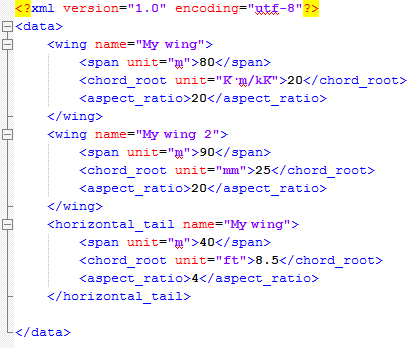
\includegraphics[height=6cm]{Immagini/xml5.png}\hfil
%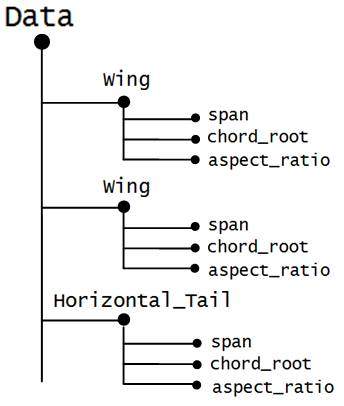
\includegraphics[height=6cm]{Immagini/xml3.jpg}
%\caption{Tree structure of an .XML file.}
%\end{figure}

%\subsection{Data Managment from XML file.}
In order to read an XML file it is necessary, first of all, to give the file path. The class \texttt{JPADXmlReader} opens the file and  the methods of the class \texttt{MyXMLReaderUtils} read the useful data from the XML having the tag path as input. It is possible to read data as \texttt{Amount}, namely with units of measurement or as \texttt{double}. The unit of measurement is written in the attributes of data in XML file.\\ 

Likewise it is possible to write output data on XML file using \texttt{JPADDataWriter} class. First of all it is necessary to define and build the xml tree structure. After each variable is associated with a name that is the markup symbol of the XML file.

%possibili sviluppi futuri

\section {Default Aircraft}
At the moment it is possible to define two different aircrafts in order to test the functionality of the application: {\bfseries ATR-72}  and {\bfseries B747-100B}. \\ \\

The {\bfseries ATR 72} is a twin-engine turboprop made by the French-Italian aircraft manufacturer ATR entered service in 1989.  It was developed as a variant of the ATR 42  with a 4.5 m stretched fuselage.  The ATR 72 was developed from the ATR 42 in order to increase the seating capacity (48 to 66 in standard configuration) by stretching the fuselage, increasing the wingspan, adding more powerful engines, and increasing fuel capacity by approximately 10 percent. It has been typically employed as a regional airliner, although other roles have been performed by the type such as corporate transport, cargo aircraft and maritime patrol aircraft. \cite{wiki:atr}


\begin{figure}[H]
\centering
{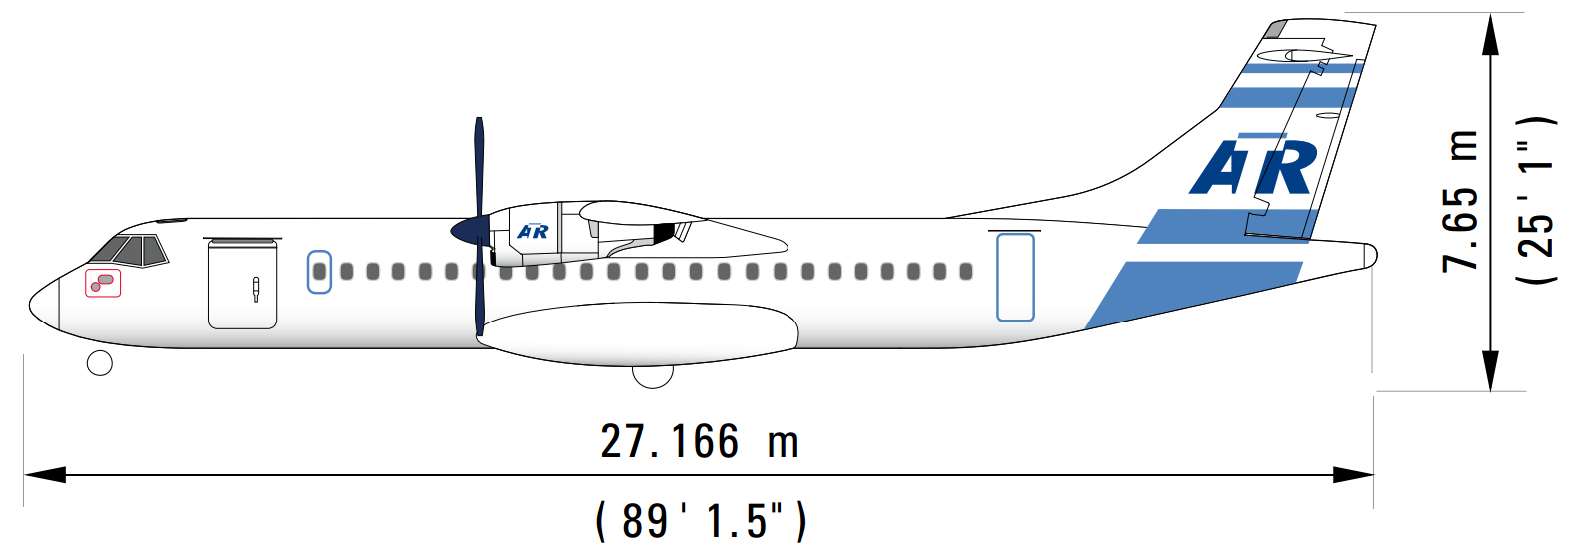
\includegraphics[height=4cm]{Immagini/atr72mod.jpg}} 
\caption{ATR 72. Side view.}
\end{figure}


The {\bfseries Boeing 747-100B} is a four-engined long-range widebody commercial jet airliner and cargo aircraft  produced by the American manufacturer Boeing Commercial Airplanes. It has a capacity of maximum 480 passengers in a partial double deck configuration. The Boeing 747 is also known as Jumbo Jet. The basic B747-100 entered service with Pan American On January 15, 1970.\\
One of the reasons to create the 747 was reductions in airfares with a consequent increase of passenger traffic\cite{wiki:boeing}. The original version of the 747 had two and a half times greater capacity than the Boeing 707, one of the common large commercial aircraft of the 1960s and it was the largest passenger carrier from 1970 until the introduction of Airbus A380.
The Boeing 747 has two aisles and four wing-mounted engines. The upper deck is its distinctive "hump" along the forward part of the aircraft. It provides space for a lounge or extra seating. The raised cockpit allows front loading of cargo on freight variants. \\
The 747-100B model was developed from the 747-100SR. This configuration has a typical 452 passengers and unlike the original 747-100, the 747-100B was offered with Pratt \& Whitney JT9D-7A, General Electric CF6-50, or Rolls-Royce RB211-524 turbofan engines.

\begin{figure}[H]
\centering
{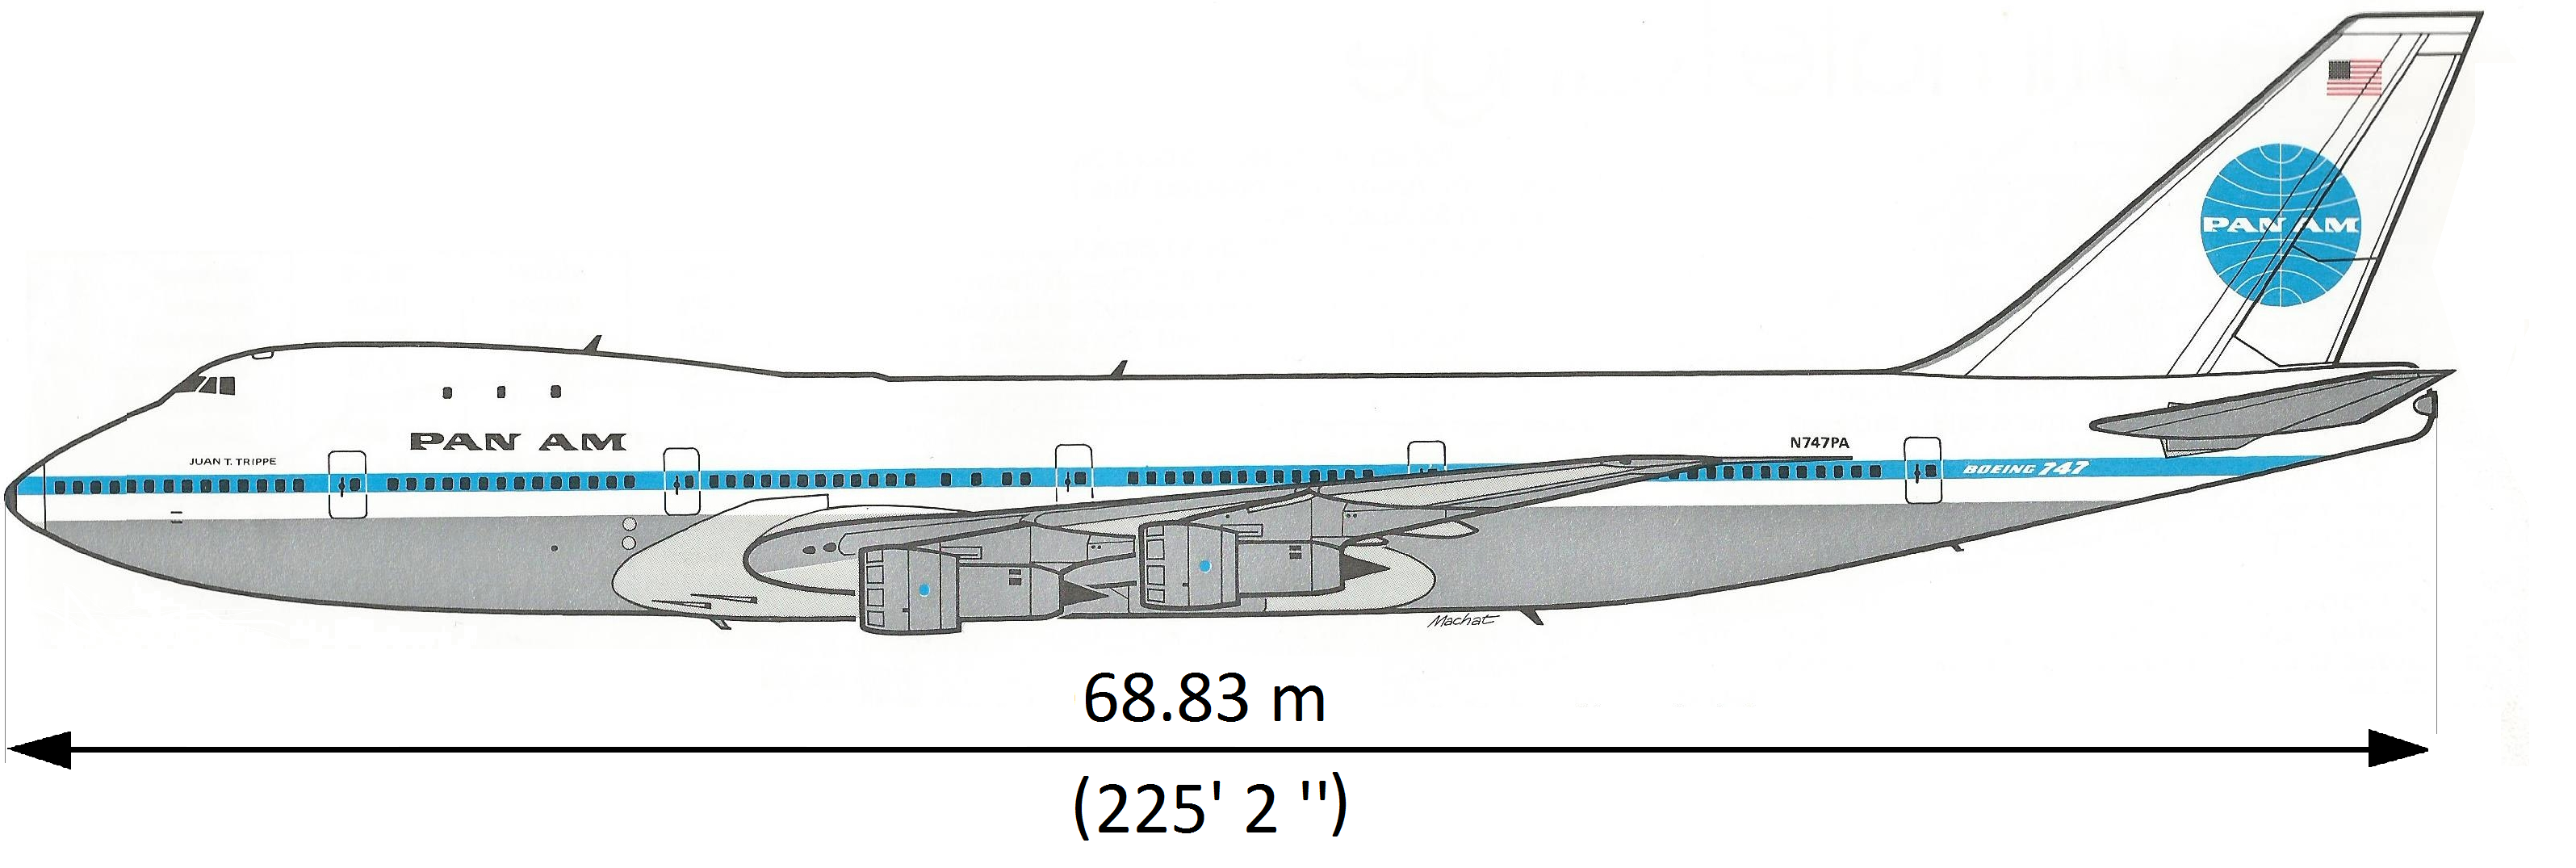
\includegraphics[height=4cm]{Immagini/boeing.jpg}} 
\caption{Boeing 747-100B. Side view.}
\end{figure}

\subsection {How is made a default Aircraft}
In order to define a Default Aircraft in a test class, and use it to check the functionalities of the application, it is necessary to follow some steps. First of all it is necessary to initialize the working directory tree using the method \texttt{initWorkingDirectoryTree} of \texttt{MyConfiguration} class located in \texttt{JPADConfigs} package that initializes the working directory tree and fills the map of folders. 
This step is required in order to create the following default folders that are necessary for the right behavior of the code:

\begin{itemize}
\item Database directory
\item Input directory
\item Output directory
\end{itemize}

Using  \texttt{MyConfiguration} class is possible to point at a specific folder, like the input or output directory, with the static method  \texttt{getDir}. This is a crucial step that must be executed at the beginning of every test.
To set the working directory with the useful folders, is necessary to call the function \texttt{initWorkingDirectoryTree()} at the beginning of each test. The function creates all necessary folders. Morover the function has been overloaded and it can be even called with a variable number of arguments (\texttt{initWorkingDirectoryTree( String...str)}). These strings are the directory strings in \texttt{MyConfiguration} class.
The second step is the creation of an\texttt{Aircraft} object choosing between the ones grouped into a dedicated \texttt{Enum}, named \texttt{AircraftEnum}.
After it is possible to create an \texttt{Aircraft} using the method \texttt{createDefaultAircraft} from \texttt{Aircraft} class. This method defines a new Aircraft object and invokes another Aircraft's method that creates the components using default data. In the method \texttt{createDefaultAircraft} there is a calling to the builder of \texttt{Aircraft} class that initializes the objects of the classes that perform calculations. At this step all the components of the aircraft are created. It is possible also to define new airfoils for the aircraft or change some data from the existing. \\
Afterwards it is necessary to set the operating conditions such as the number of Mach of analysis or altitude. Each default aircraft has a set of default conditions but the user could change them.\\
In order to manage all the aircraft related analyses it is necessary to define an object of the class  \texttt{ACAnalysisManager}. Similarly to the aircraft, an analysis manager  exists also for the wing that is an object of the  \texttt{LSAerodynamicManager} class. \\
The next step is to define and assign the needed databases. This will be explained in detail in the next section. Finally it is possible to do analysis.

\noindent \\
\begin{lstlisting}[frame=rbl,caption={{\footnotesize Generation of default aircraft}},label= [style=\bfseries]{Listing}]
public static void main(String[] args) {

	// --------------------------------------------------------------
	// Define directory
	// --------------------------------------------------------------
	MyConfiguration.initWorkingDirectoryTree();


	// --------------------------------------------------------------
	// Generate default Aircraft
	// --------------------------------------------------------------
	Aircraft aircraft = Aircraft.createDefaultAircraft(AircraftEnum..B747_100B);
	LiftingSurface theWing = aircraft.get_wing();

	// Default operating conditions
	OperatingConditions theConditions = new OperatingConditions();		


	// --------------------------------------------------------------
	// Define an ACAnalysisManager Object
	// --------------------------------------------------------------
	ACAnalysisManager theAnalysis = new ACAnalysisManager(theConditions);
	theAnalysis.updateGeometry(aircraft);


	// --------------------------------------------------------------
	// Define an LSAerodynamicsManager Object
	// --------------------------------------------------------------
	LSAerodynamicsManager theLSAnalysis = new LSAerodynamicsManager ( 
			theConditions,
			theWing,
			aircraft
			);

		
	// --------------------------------------------------------------
	// Setup database(s)	
	// --------------------------------------------------------------
		
	theLSAnalysis.setDatabaseReaders(
			new Pair(DatabaseReaderEnum.AERODYNAMIC,
                          "Aerodynamic_Database_Ultimate.h5"),
			new Pair(DatabaseReaderEnum.HIGHLIFT,  
                          "HighLiftDatabase.h5")
			);

	
	// --------------------------------------------------------------
	// Do analysis
	// --------------------------------------------------------------
	theAnalysis.doAnalysis(aircraft, 
			AnalysisTypeEnum.AERODYNAMIC);
}
\end{lstlisting}

\begin{sidewaysfigure}

\centering
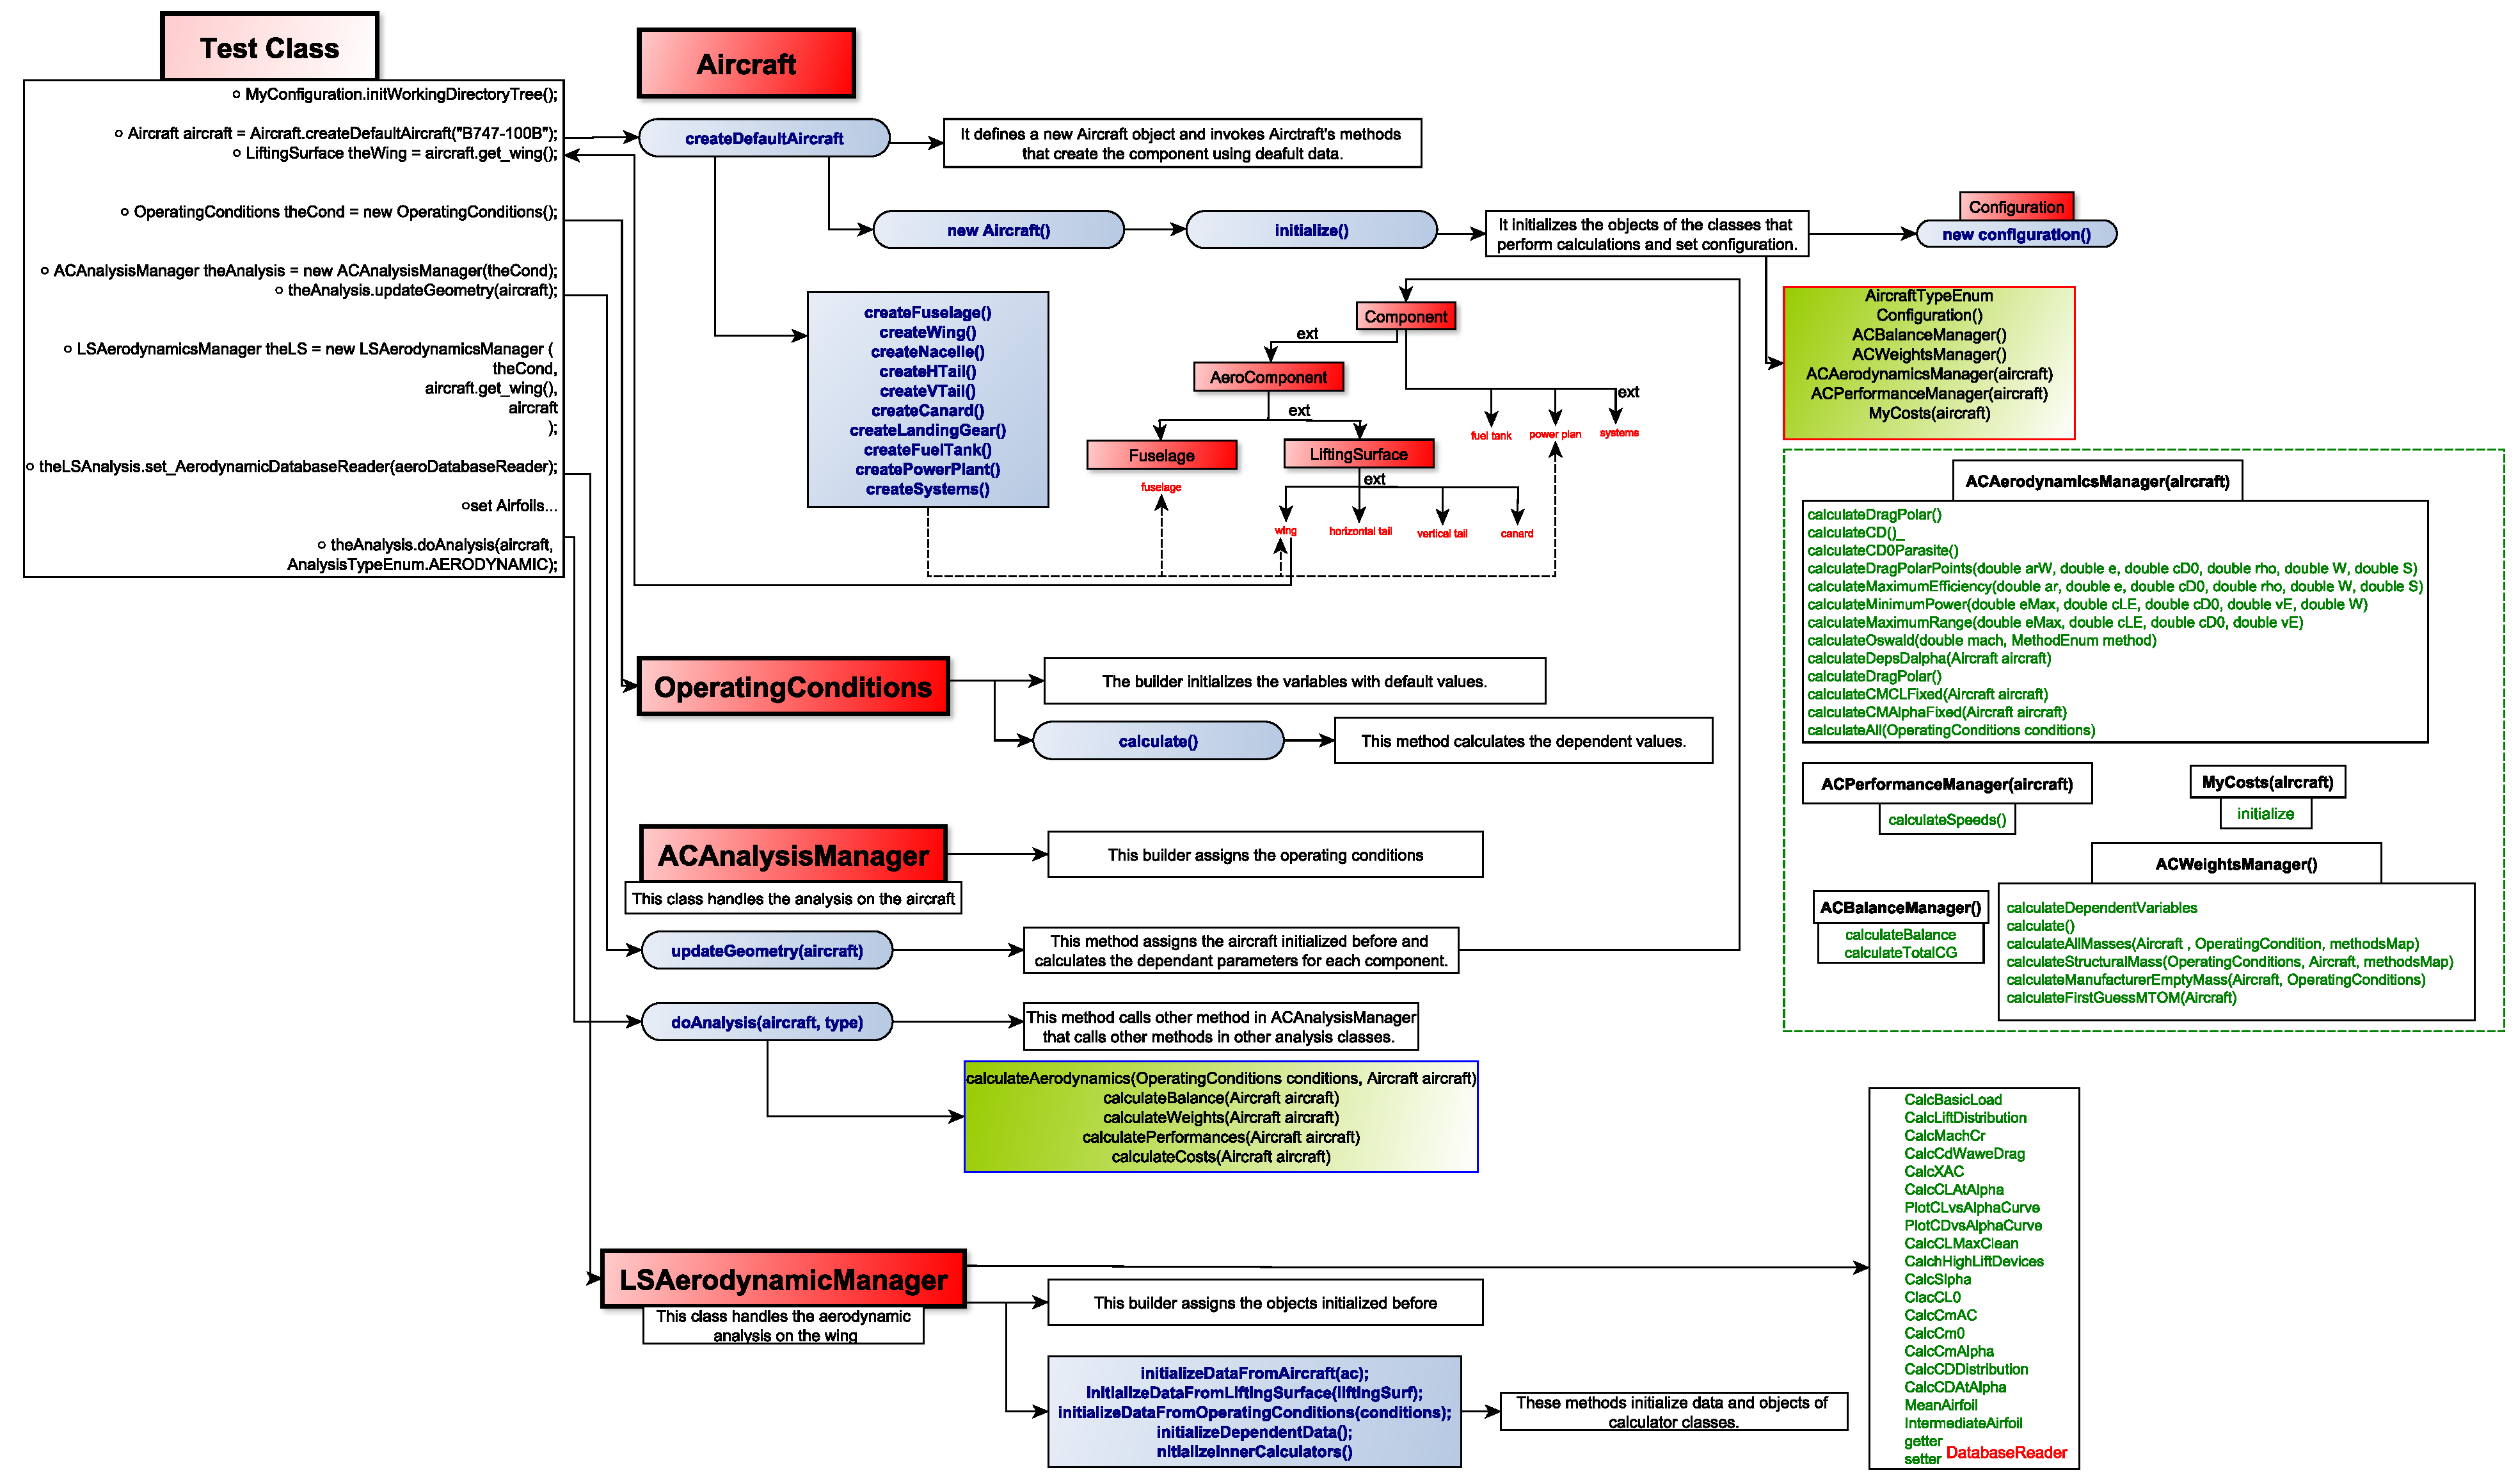
\includegraphics[width=24.6cm]{immagini/HowToCreateADefaultAircraftInJPAD3.pdf}
\caption{Flow chart of the creation of default Aircraft.}
\label{fig:schemauno}

\end{sidewaysfigure}

\subsection {How is made a default Wing}
Similary to the default aircraft it is possible to define a default wing. This is very useful if the user wants to make an analysis only on a wing. In this case it is necessary to define the origin of the \gls{acr:lrf} in \gls{acr:brf} and the coordinates of the \gls{acr:cg}.\\
Contrary to the case of the aircraft, for an isolated wing it is not necessary to define a fuselage in order to create a \texttt{Lifting Surface} object, but there is an overload of the builder that does not need a fuselage as input. In this case the exposed surface is calculated as the surface of the wing.

\noindent \\
\begin{lstlisting}[frame=rbl,caption={{\footnotesize Generation of an isolated Wing}},label= [style=\bfseries]{Listing}]
public static void main(String[] args) {

	// Assign all default folders
	MyConfiguration.initWorkingDirectoryTree();
	
	// -----------------------------------------------------------------------
	// Coordinates of LRF
	// -----------------------------------------------------------------------
	
	double xAw = 11.0; //meter 
	double yAw = 0.0;
	double zAw = 1.6;
	double iw = 0.0;
	
	// -----------------------------------------------------------------------
	// Generate default Wing
	// -----------------------------------------------------------------------
	
	LiftingSurface theWing = new LiftingSurface(
			"Wing", // name
			"Data from AC_ATR_72_REV05.pdf", 
			xAw, yAw, zAw, iw, 
			ComponentEnum.WING
			); 

	theWing.calculateGeometry();
	theWing.getGeometry().calculateAll();
	
	// -----------------------------------------------------------------------
	// Center of Gravity
	// -----------------------------------------------------------------------	
	
	double xCgLocal= 1.5; // meter 
	double yCgLocal= 0;
	double zCgLocal= 0;

	CenterOfGravity cg = new CenterOfGravity(
			Amount.valueOf(xCgLocal, SI.METER), // coordinates in LRF
			Amount.valueOf(yCgLocal, SI.METER),
			Amount.valueOf(zCgLocal, SI.METER),
			Amount.valueOf(xAw, SI.METER), // origin of LRF in BRF 
			Amount.valueOf(yAw, SI.METER),
			Amount.valueOf(zAw, SI.METER),
			Amount.valueOf(0.0, SI.METER),// origin of BRF
			Amount.valueOf(0.0, SI.METER),
			Amount.valueOf(0.0, SI.METER)
			);

	cg.calculateCGinBRF();
	theWing.set_cg(cg);
	theWing.set_aspectRatio(6.0);

	// Default operating conditions
	OperatingConditions theOperatingConditions = new OperatingConditions();		
	theOperatingConditions.set_alphaCurrent(Amount.valueOf(2.0, NonSI.DEGREE_ANGLE)

	// --------------------------------------------------------------
	// Define an LSAerodynamicsManager Object
	// --------------------------------------------------------------
	
	LSAerodynamicsManager theLSAnalysis = new LSAerodynamicsManager ( 
			theOperatingConditions,
			theWing
			);

	// --------------------------------------------------------------
	// Setup database(s)	
	// --------------------------------------------------------------
	
	theLSAnalysis.setDatabaseReaders(
			new Pair(DatabaseReaderEnum.AERODYNAMIC, 
					"Aerodynamic_Database_Ultimate.h5"),
			new Pair(DatabaseReaderEnum.HIGHLIFT, "HighLiftDatabase.h5")
			);
	
	// --------------------------------------------------------------
	// Assign Airfoil(s) ...	
	// --------------------------------------------------------------

	  // Define airfoilRoot...
	
	// --------------------------------------------------------------
	// Set Airofoil(s)	
	// --------------------------------------------------------------
	List<MyAirfoil> myAirfoilList = new ArrayList<MyAirfoil>();
	myAirfoilList.add(0, airfoilRoot);
	myAirfoilList.add(1, airfoilKink);
	myAirfoilList.add(2, airfoilTip);
	theWing.set_theAirfoilsList(myAirfoilList);
	theWing.updateAirfoilsGeometry(); 
	theLSAnalysis.initializeDependentData();

}
\end{lstlisting}

\section {Database in JPAD}

In JPAD it is possible to consult external databases in .h5 format. {\bfseries HDF 5} (Hierarchical Data Format Release 5) is a data file format designed by the {\itshape National Center for Supercomputing Applications} (NCSA) to assist users in the storage and manipulation of scientific data across different operating systems and machines.\\
To obtain the useful data in JPAD  interpolating functions are used . These functions can be of one, two or three dimensions and read data from graphics that have been digitize previously.\\
Starting from these digitalizations, databases in .h5 format are built.
Reading data from databases is entrusted to methods of classes in the \texttt{database} package.\\
In order to read these databases, and obtain the useful data, it is necessary to define an object of the database reading class and associate it with the object of analysis.\\
This is a crucial step to read correctly the external data. Infact JPAD allows to work with an aircraft object  or only with an isolated lifting surface object.  Aircraft is usually composed of a fuselage, lifting surfaces, nacelle and power plant.
Furthermore, \texttt{Aircraft} and \texttt{Wing} are associated with classes of calculation like \texttt{LSAerodynamicManager} or \texttt{ACAnalysisManager}. So it is necessary that these databases are also visible from these classes.\\
So because both in the aircraft and in the wing there is a lifting surface object, databases relative to wing are associated to \texttt{LSAerodynamicManager}.

\subsection {Setup database}
Here the database path is created and associated to object that interpolates the required data from the .h5 file using a \texttt{MyInterpolatingFunction} object. After this it is possible to access the double value of the interpolating function using the \texttt{standaloneutils} method called \texttt{value}. \\


%\begin{lstlisting}[frame=rbl,caption={{\footnotesize Setup database(s)}},label= [style=\bfseries]{Listing}]
%// --------------------------------------------------------------
%// Define database
%// --------------------------------------------------------------
%MyConfiguration.initWorkingDirectoryTree();
%
%// Setup database(s)	
%String databaseFolderPath = MyConfiguration.getDir(FoldersEnum.DATABASE_DIR);
%String databaseFileName = "Aerodynamic_Database_Ultimate.h5";
%AerodynamicDatabaseReader aeroDatabaseReader = 
%		new AerodynamicDatabaseReader(
%				databaseFolderPath, 
%				databaseFileName
%				);
%\end{lstlisting}

Now the procedure to assign the database is different if is used an Aircraft object or a Wing object.

\subsection {Assign database using an Aircraft object}
In order to assign correctly the database and associate it to all analysis management is necessary to practise the following order.
\begin{enumerate}
\item Define an Aircraft Object.\\This command associates to the Aircraft an object that defines the aerodynamic. Defining an Aircaft object is defined the Wing, that is a \texttt{LiftingSurface} object.
\item Define an \texttt{ACAnalysisManager} object.\\All the aircraft computations are managed by this class.
\item Define an \texttt{LSAerodynamicManager} object.\\ All the lifting surfaces computations are managed by this class.
\item Associate database to \texttt{LSAerodynamicManager}.
\item Eventually do analysis.
\end{enumerate}

\subsection {Assign database using a Wing object}
Using a Wing object it is not necessary to define a manager for Aircraft aerodynamic analysis. So the step to follow are the same of aircraft starting from the third.
\begin{enumerate}
\item Define a Wing Object.
\item Define an \texttt{LSAerodynamicManager} object.
\item Associate database to \texttt{LSAerodynamicManager}.
\end{enumerate}

The definition of an isolated Wing is explained in the relative section.

%\begin{lstlisting}[frame=rbl,caption={{\footnotesize Assign database using an Aircraft object}},label= [style=\bfseries]{Listing}]
%
%// --------------------------------------------------------------
%// Generate default Aircraft
%// --------------------------------------------------------------
%Aircraft aircraft = Aircraft.createDefaultAircraft("B747-100B");
%LiftingSurface theWing = aircraft.get_wing();
%		
%// Default operating conditions
%OperatingConditions theConditions = new OperatingConditions();		
%		
%		
%// --------------------------------------------------------------
%// Define an ACAnalysisManager Object
%// --------------------------------------------------------------
%ACAnalysisManager theAnalysis = new ACAnalysisManager(theConditions);
%theAnalysis.updateGeometry(aircraft);
%		
%		
%// --------------------------------------------------------------
%// Define an LSAerodynamicsManager Object
%// --------------------------------------------------------------
%LSAerodynamicsManager theLSAnalysis = new LSAerodynamicsManager ( 
%		theConditions,
%		theWing,
%		aircraft
%		);
%		
%		
%// --------------------------------------------------------------
%// Associate database to LSAerodynamicManager
%// --------------------------------------------------------------
%theLSAnalysis.set_AerodynamicDatabaseReader(aeroDatabaseReader);
%
%		
%// --------------------------------------------------------------
%// Do analysis
%// --------------------------------------------------------------
%theAnalysis.doAnalysis(aircraft, 
%		AnalysisTypeEnum.AERODYNAMIC);
%\end{lstlisting}

\noindent \\
\begin{lstlisting}[frame=rbl,caption={{\footnotesize Assign database using an Aircraft object}},label= [style=\bfseries]{Listing}]
		
	// --------------------------------------------------------------
	// Setup database(s)	
	// --------------------------------------------------------------
		
	theLSAnalysis.setDatabaseReaders(
			new Pair(DatabaseReaderEnum.AERODYNAMIC,
                          "Aerodynamic_Database_Ultimate.h5"),
			new Pair(DatabaseReaderEnum.HIGHLIFT,  
                          "HighLiftDatabase.h5")
			);

\end{lstlisting}
The databases are assigned to \texttt{LSAerodynamic} using a method of this class. This method accept as input a variable number of \texttt{Pair} objects.Using \texttt{Pair} objects it is possible to assign, for each database, both name and type. 

\noindent \\
\begin{lstlisting}[frame=rbl,caption={{\footnotesize \texttt{setDatabaseReaders} method}},label= [style=\bfseries]{Listing}]

public void setDatabaseReaders(Pair... args) {
	String databaseFolderPath = MyConfiguration.getDir(FoldersEnum.DATABASE_DIR);
	
	for (Pair a : args) {
		DatabaseReaderEnum key = (DatabaseReaderEnum)a.getKey(); 
		String databaseFileName = (String)a.getValue();
		
		switch (key) {
			case AERODYNAMIC:
				_aerodynamicDatabaseReader = 
				new AerodynamicDatabaseReader(
						databaseFolderPath,
						databaseFileName); 
				listDatabaseReaders.add(_aerodynamicDatabaseReader);
				break;
				
			case HIGHLIFT:
				_highLiftDatabaseReader = 
				new HighLiftDatabaseReader(
						databaseFolderPath, 
						databaseFileName); 
				listDatabaseReaders.add(_highLiftDatabaseReader);
			break;	
			
		}
\end{lstlisting}


\subsection {User's guide}

In order to execute some analysis in JPAD it is necessary, first of all, to define an analysis object in the Test class. The method \texttt{createDefaultAircraft} creates a new aircraft and the object that composes it. This method also populates the data of aircraft with default value corresponding to ATR-72 or Boieng 747-100B. Moreover the method \texttt{createDefaultAircraft} calls another method in \texttt{Aircraft} class: \texttt{initialize} that initializes the objects of the classes that perform calculations. \\
The purpose of this structure is to have only a way to assign the databases at an aircraft. Inasmuch as the wing is always present, the chosen strategy is to assign the database to the aerodynamic manager of the wing.\\
In order to bring to use the database also for the aircraft calculation, it is assigned at the aerodynamic manager of the aircraft in the method called \texttt{doAnalysis}.\\
At the same time \texttt{LSAerodynamicManager} sets itself as aerodynamic in the wing object. \\
So it is possible to call the database using equally the following codes: 
\begin{itemize}
\item \texttt{theWingObject.getAerodynamics.get\_Database;}
\item \texttt{theAircraftObject.get\_theAerodynamic.get\_Database;}
\item \texttt{theLSManagerObject.get\_Database;}
\item \texttt{theACManagerObject.get\_Database;}
\end{itemize}

\begin{sidewaysfigure}

\centering
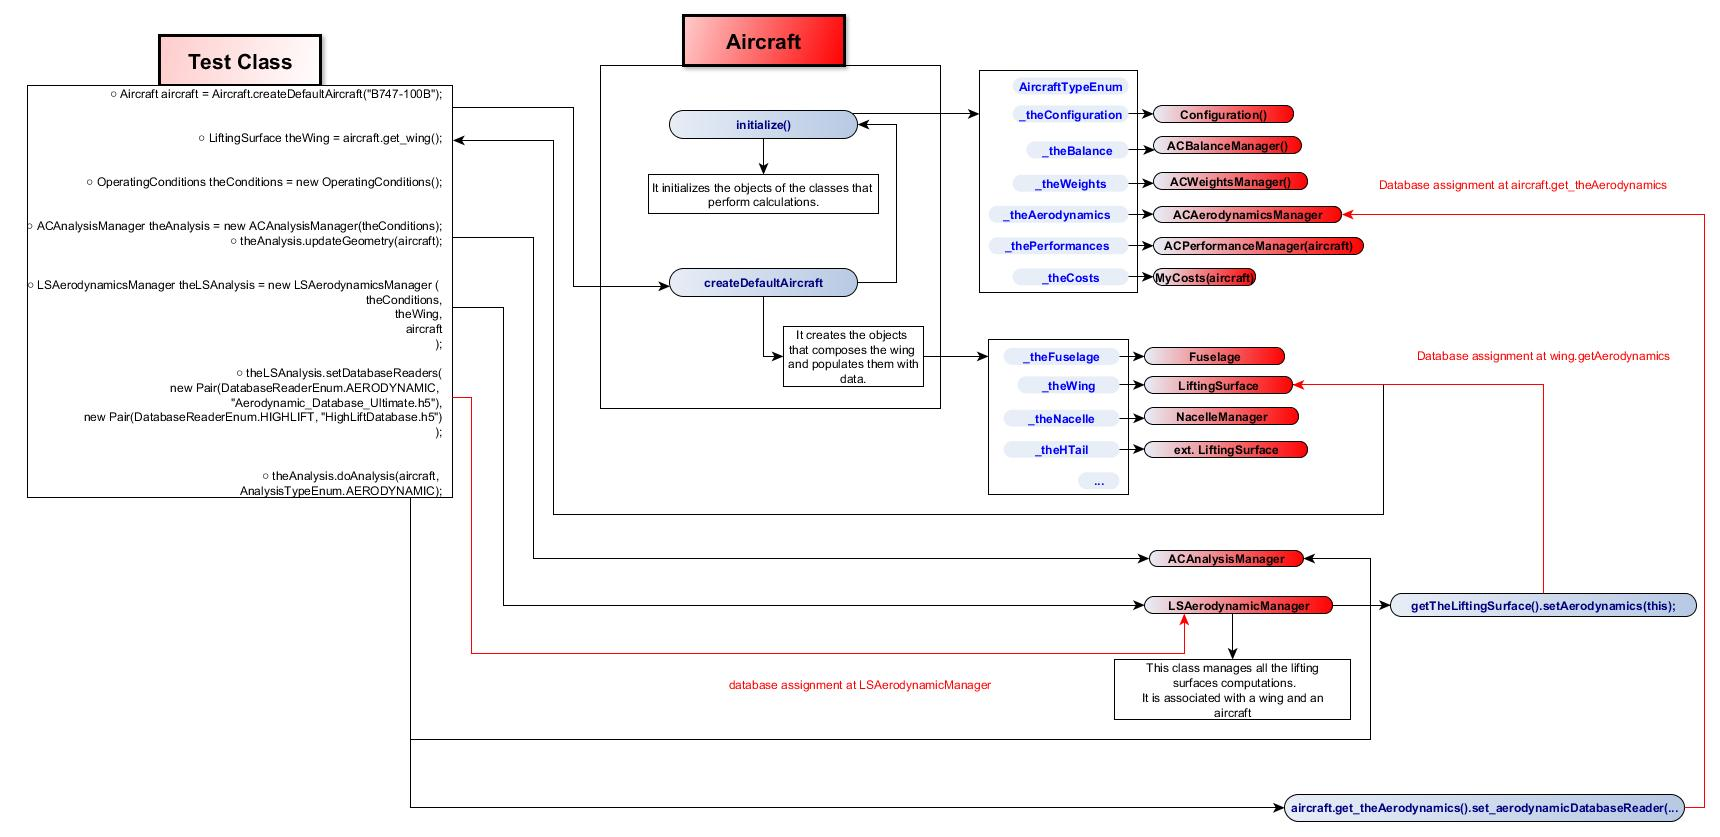
\includegraphics[width=23cm]{immagini/HowToAssignDatabase.jpg}
\caption{Flow chart of database assignment.}
\label{fig:schemauno}

\end{sidewaysfigure}

% -----------------------------------------------------------------------------------------
%                                                                A P P E N D I C I
% -----------------------------------------------------------------------------------------

\appendix
%\input{appendice1}



\backmatter % materiale finale( bibliografia, risorse utilizzate)



% -----------------------------------------------------------------------------------------
%                                                                L I S T A   D E I   S I M B O L I   E   G L O S S A R I O 
% -----------------------------------------------------------------------------------------

% -----------------------------------------------------------------------------------------
%                                                               A C R O N I M I 
% -----------------------------------------------------------------------------------------

% -----------------------------------------------------------------------------------------
%                                                               B I B L I O G R A F I A
% -----------------------------------------------------------------------------------------

%\input{biblio}

\end{document}